% ****** Start of file apssamp.tex ******
%
%   This file is part of the APS files in the REVTeX 4.2 distribution.
%   Version 4.2a of REVTeX, December 2014
%
%   Copyright (c) 2014 The American Physical Society.
%
%   See the REVTeX 4 README file for restrictions and more information.
%
% TeX'ing this file requires that you have AMS-LaTeX 2.0 installed
% as well as the rest of the prerequisites for REVTeX 4.2
%
% See the REVTeX 4 README file
% It also requires running BibTeX.
% The commands are as follows:
%
%  1)  latex apssamp.tex
%  2)  bibtex apssamp
%  3)  latex apssamp.tex
%  4)  latex apssamp.tex
%
\RequirePackage{fix-cm}
% Preserve the modern hook-aware label command across REVTeX's older override.
\let\latexKernelLabel\label
\documentclass[%
 reprint,
%superscriptaddress,
%groupedaddress,
%unsortedaddress,
%runinaddress,
%frontmatterverbose,
%preprint,
%preprintnumbers,
%nofootinbib,
%nobibnotes,
%bibnotes,
 amsmath,amssymb,
 superscriptaddress,
 aps,
prl,
floatfix,
%prb,
%rmp,
%prstab,
%prstper,
%floatfix,
]{revtex4-2}

% Keep local filenames literal so editors can collect the document's assets.
% Repository-root latexmk builds resolve them through latexmkrc.

\DeclareRobustCommand{\timesbox}{%
  \mathbin{%
    \scalebox{0.8}{
    \ooalign{%
      $\Box$\cr
      \hfil\raisebox{0.2ex}{$\times$}\hfil\cr % move up
    }%
    }
  }%
}
\usepackage{booktabs}
\usepackage{multirow}
\usepackage{slashed}
\usepackage[normalem]{ulem}
\usepackage{graphicx}% Include figure files
\usepackage{dcolumn}% Align table columns on decimal point
\usepackage{bm}% bold math
% REVTeX places footnotes in the bibliography, so its footnote patch is unused.
\usepackage[nopatch=footnote]{microtype}
\hyphenation{had-ro-pro-duc-tion}

\usepackage{braket}
\usepackage{etoolbox}
\makeatletter
\IfFormatAtLeastTF{2023-06-01}{%
  \let\label\latexKernelLabel
  \let\ltx@label\label
}{}
% Supply REVTeX's effective author flags explicitly and retain textual years.
% The author control is hexadecimal: 48 = initials (08) + journal order (40).
\newcommand{\patchAPSBibControl}[2]{%
  \patchcmd{\@bibdataout@aps}{#1}{#2}{}{%
    \PackageError{ludy-paper}{REVTeX bibliography control patch failed}%
      {Check the installed REVTeX bibliography control definition.}%
  }%
}
% Patch both the long- and short-bibliography branches.
\patchAPSBibControl{author="08"}{author="48"}
\patchAPSBibControl{author="08"}{author="48"}
\patchAPSBibControl{year="1"}{year="0"}
\patchAPSBibControl{year="1"}{year="0"}
\makeatother
\usepackage{hyperref}
% Let arXiv labels wrap after the prefix without changing their link targets.
\newcommand{\Eprint}[2]{%
  \begingroup
  \def\eprintText{#2}%
  \patchcmd{\eprintText}{arXiv:}{arXiv:\allowbreak}{}{}%
  \href{#1}{\eprintText}%
  \endgroup
}
\usepackage[table]{xcolor}
% Reviewer comments transcribed from LUDY-1790769002675.pdf.
\definecolor{ValentinComment}{RGB}{112,42,145}
\DeclareRobustCommand{\valentin}[1]{%
  \textcolor{ValentinComment}{[\textbf{Valentin:} #1]}%
}
\definecolor{LucienComment}{RGB}{35,125,95}
\DeclareRobustCommand{\lucien}[1]{%
  \textcolor{LucienComment}{[\textbf{Lucien:} #1]}%
}

\definecolor{ZenoComment}{RGB}{35,110,135}
\DeclareRobustCommand{\zeno}[1]{%
  \textcolor{ZenoComment}{[\textbf{Zeno:} #1]}%
}
% %
%
%
%
%
% %
%
%
%
%
\usepackage{pgfplots} 
\pgfplotsset{compat=1.18}
\usepackage{cleveref}
\usepackage{fancyvrb}
\usepackage{ragged2e}
\newcommand{\topblackrule}{%
  \noalign{\color{black}\hrule height 0.65pt}%
}
\newcommand{\midblackrule}{%
  \noalign{\color{black}\hrule height 0.40pt}%
}
\newcommand{\bottomblackrule}{%
  \noalign{\color{black}\hrule height 0.65pt}%
}

\definecolor{ludybg}{RGB}{232,243,247}   % very light blue-cyan
\definecolor{refbg}{RGB}{248,238,230}    % very light peach
\definecolor{mgfivebg}{RGB}{248,238,230} % very light peach
\usetikzlibrary{patterns}
\allowdisplaybreaks
\begin{document}


\title{The KLN theorem meets collinear factorisation: \texorpdfstring{\\}{ }Local Unitarity for Hadronic Cross-Sections}%
%


\author{Zeno Capatti}
%\email{zeno.capatti@unibe.ch}
\affiliation{%
CERN, Theory Department, 1211 Geneva 23, Switzerland
}
\affiliation{%
  Institute for Theoretical Physics, University of Bern, 3012 Bern, Switzerland
}

\author{Lucien Huber}
%\email{Second.Author@institution.edu}

% This applies to both preceding authors:
\affiliation{%
  Institute for Theoretical Physics, University of Bern, 3012 Bern, Switzerland
}


%\author{Michael Ruf}
% \email{Second.Author@institution.edu}
%\affiliation{SLAC National Accelerator Laboratory, \\ Stanford University, \\ Stanford, CA 94039}

%\date{\today}% It is always \today, today,
             %  but any date may be explicitly specified

\begin{abstract}
We present an initial-state implementation of the Kinoshita--Lee--Nauenberg (KLN) theorem that is compatible with collinear factorisation.
In this formulation, hadronic cross-sections are expressed as convolutions of parton distribution functions with partonic cross-sections obtained by summing over the number of incoming partons.
By virtue of the KLN theorem, the partonic cross-sections are infrared finite without requiring infrared renormalisation.
The Local Unitarity formalism provides a local realisation of this infrared finiteness, allowing partonic cross-sections to be evaluated directly in four dimensions by Monte Carlo integration.
We demonstrate the framework at next-to-leading order and leading power.
Using Local Unitarity, we compute the Drell--Yan and $t\bar{t}$ production cross-sections numerically; using Reverse Unitarity, we obtain the deep inelastic scattering and Drell--Yan cross-sections analytically. In all cases, a universal scheme conversion relates our results to those obtained in the conventional \(\overline{\mathrm{MS}}\) parton model.

\end{abstract}

%\keywords{Suggested keywords}%Use showkeys class option if keyword
                              %display desired
\maketitle

%\tableofcontents

\section{Introduction}
\label{sec:introduction}

Producing meaningful perturbative predictions for hadronic collisions requires connecting the scattering of asymptotic quarks and gluons to that of hadrons. A consistent framework must ensure infrared (IR) finiteness, allow systematic resummation of large logarithms arising from soft and collinear radiation, and provide a universal description of the nonperturbative structure of hadrons.

In conventional calculations of hadronic cross-sections, infrared finiteness relies on two complementary mechanisms. Final-state infrared singularities cancel upon summing over the number of degenerate final-state massless particles, as guaranteed by the Kinoshita--Lee--Nauenberg (KLN) theorem~\cite{Kinoshita:1962ur,PhysRev.133.B1549}. The number of initial-state partons is instead kept fixed, breaking the KLN mechanism. Collinear factorisation~\cite{PhysRevD.8.3633,DAVIDPOLITZER1974129,Altarelli:1979ub,Collins:1981ta,Collins:1981tt,Collins:1983ju,Collins:1983pk,Collins:1985ue,Collins:1989gx,Bodwin:1984hc,Ellis:1978ty} provides a complementary mechanism: initial-state collinear singularities factorise universally and are absorbed into the renormalisation of parton distribution functions (PDFs), while soft singularities associated with initial--initial and initial--final dipoles cancel separately between real and virtual contributions. This asymmetric treatment raises the question of whether the KLN theorem can also be implemented in the initial state while preserving collinear factorisation.

In this paper, we investigate an initial-state implementation of the KLN theorem in which partonic cross-sections are defined by summing over degenerate initial- and final-state configurations of different massless-parton multiplicities, ensuring KLN-driven cancellation of infrared singularities in both states. Within the Local Unitarity (LU) framework~\cite{Capatti:2020xjc,Capatti:2021bsm,Capatti:2022tit,Capatti:2025khs}, these cancellations can be realised locally, enabling direct Monte Carlo integration of partonic cross-sections in four dimensions. We demonstrate our framework at next-to-leading order (NLO), computing the deep inelastic scattering (DIS) and Drell--Yan (DY) cross-sections analytically using Reverse Unitarity~\cite{Anastasiou:2002qz,Anastasiou:2002yz,Anastasiou:2003yy,Anastasiou:2013mca,Anastasiou:2013srw}, while Drell--Yan and $t\bar{t}$ production cross-sections are computed numerically using Local Unitarity.

At leading power in a virtuality expansion unique to our framework, partonic cross-sections are IR-finite without the need for a renormalisation procedure, evolve according to DGLAP equations~\cite{Altarelli:1977zs,Dokshitzer:1977sg,Gribov:1968ia,Gribov:1972ri} and turn into their $\overline{\text{MS}}$ parton model counterparts by a universal redefinition of the PDFs. Hence, we reconcile for the first time an initial-state implementation of the KLN theorem with collinear factorisation.
In turn, this framework provides a new way to compute $\overline{\text{MS}}$ hadronic cross-sections, and offers a systematic method for studying subleading power contributions.
% Valentin PDF: page 1, annotation 454.
%\valentin{“natural” is a weird word here.
%Maybe “in the particular virtuality \ldots{}” instead?}
% Valentin PDF: page 1, annotation 456.
%\valentin{two sentences here.
%Starting with: 
%“The resulting preductions still evolve according to\ldots{}”}

%First, the KLN-finite cross-section is computed within the LU approach in four dimensions using Monte Carlo methods.
%Then, the numerical cross-section is converted to the $\overline{\text{MS}}$ scheme by adding a universal, analytically precomputed scheme-changing counterterm.



\section{Simplest clustering criterion}
\label{sec:clustering}

In order to relate the scattering of many partons with that of hadrons, we introduce the \emph{simplest clustering criterion}, which answers the question: ``What is the most analytically tractable definition of jet clustering?'', thus guaranteeing that calculations within our formalism may be done analytically with existing techniques.
%

Consider $n$ massless partons and the usual Lorentz-invariant phase-space measure ($d=4-2\epsilon$):
\begin{equation}
\mathrm{d}\Pi_n=\prod_{i=1}^{n} \frac{\mathrm{d}^d q_i}{(2\pi)^{d-1}} \delta(q_i^2)\Theta(q_i^0).
\end{equation}
% Valentin PDF: page 1, annotation 460.
\valentin{Funnily enough I think that technically $\Theta(q_i^0)$ is only Lorentz invariant because the partons are massless. But no need to stress that ofc.} {\color{red} Lorentz group is not simply connected. This measure is invariant under the ortochronous lorentz group.}
%
The $n$ partons are clustered in a compound object with momentum $p$ by the following integration measure~\cite{Capatti:2025gqj}:
\begin{equation}
\label{eq:1_clustering}
\mathrm{d}\Pi_n^\mathbf{p}=\mathrm{d}\Pi_n\frac{\delta(q_{1n}-p)\delta_{\mathfrak{a},\mathfrak{q}_{1n}}}{4\pi\langle\mathfrak{a}\rangle},
\end{equation}
with $q_{1n}=q_1+...+q_n$ and $\mathfrak{q}_{1n}=\mathfrak{q}_1+...+\mathfrak{q}_n$.
Here, $\mathbf{p}=(p,\mathfrak{a})$ is the tuple of the momentum $p$ of the cluster and its quark number $\mathfrak{a}\in\mathbb{Z}$.
The quark number of the $i$-th parton is $\mathfrak{q}_i=1$ for a quark, $\mathfrak{q}_i=-1$ for an anti-quark, and $\mathfrak{q}_i=0$ for a gluon.
% Valentin PDF: page 2, annotation 562.
\valentin{“quark number” is a bit clunky no? Can’t you use an actual QCD-conserved charge / quantum number of the theory (e.g. hypercharge?)}{\color{red} this matches with the name used in the DIS paper. I don't see any conventional charge.}
%
%
%
Explicitly, $\langle\mathfrak{a}\rangle=2N_c$ for $\mathfrak{a}= \pm 1$ ($q,\bar{q}$), and $\langle\mathfrak{a}\rangle=(d-2)(N_c^2-1)$ for $\mathfrak{a}=0$ ($g$).
% Valentin PDF v2: page 2, annotation 1456.
\valentin{You shoudl add ghost here.}
{\color{red} we don't have ghosts in the initial state}
%
%
Equation~\eqref{eq:1_clustering} imposes that the momenta and quark numbers of the $n$ initial-state partons must sum up to the cluster's momentum $p$ and quark number $\mathfrak{a}$.
%

We cluster $n$ partons into two compound objects with momenta $p_1$ and $p_2$ by distributing them according to:
% Valentin PDF: page 2, annotation 564.
\valentin{why not “with configurations P\_bold\_1 and P\_bold\_2...” instead?}{\color{red} see new change below}
%
\begin{equation}
\label{eq:2_clustering}
\mathrm{d}\Pi_n^{\mathbf{p}_1\mathbf{p}_2}=\sum_{(S_1,S_2)\in J_n}\frac{\mathrm{d}\Pi_n}{4\pi} \prod_{j=1}^2 \frac{\delta(q_{S_j}-p_j)\delta_{\mathfrak{a}_j,\mathfrak{q}_{S_j}}}{\langle\mathfrak{a}_j\rangle},
\end{equation}
with $q_{S_i}=\sum_{j\in S_i} q_j$ and $\mathfrak{q}_{S_i}=\sum_{j\in S_i} \mathfrak{q}_j$, and
\begin{equation}
J_n=\left\{(S_1,S_2)\big|\, S_i\subset[n], \, S_1\cup S_2=[n]\right\},
\end{equation}
with $[n]=\{1,...,n\}$, and $\mathbf{p}_i=(p_i,\mathfrak{a}_i)$.
Each initial-state parton belongs to one or both clusters.
The momenta and quark numbers of all partons belonging to the $i$-th cluster must sum up to the momentum $p_i$ and quark number $\mathfrak{a}_i$.
As $p_i^2$ becomes small, the momentum of a parton contained within the $i$-th cluster will be either a) collinear to $p_i$, if it is contained only in one cluster,or  b) soft, if it is contained in both clusters.
% Valentin PDF: page 2, annotation 566.
\valentin{maybe rephrase:
“\ldots{}, the momentum of a parton becomes collinear when exclusively within a single cluster, and necessarily soft when part of both clusters.”}{\color{red} ok changed}
%
%
%

\section{Cross-sections with many initial-state partons}
\label{sec:formalism}

In DIS, a high-energy electron scatters against a proton.
% Valentin PDF: page 2, annotation 568.
\valentin{It’s more natural to me to state that a “high-energy electron scatters against a proton”}{\color{red} ok}
%
In the single-photon-exchange approximation used here {\color{red} prefer QCD corrections}, the interaction is mediated by a virtual photon with momentum $q$ emitted by the electron with momentum $p_e$.
%
The partonic cross-section is the contraction of the leptonic tensor $L_{\mu\nu}(p_e,q)$ and the partonic tensor $W_{\mathfrak{a}}^{\mu\nu}(x,q^2;\Lambda^2)$ that depends on the Bjorken variable $x$, on $q^2$, and an infrared scale $\Lambda^2$.
%
Given the collections of all partonic combinations:
% Valentin PDF: page 2, annotation 572.
\valentin{There is no ordering here, so “sequences” $\to$ “combinations”}{\color{red} ok}
%
%
\begin{equation}
 \mathfrak{S}_n=\bigcup_{j=1}^n \{q,\bar{q},g\}^j,
\end{equation}
and $\tilde{\mathfrak{S}}_n=\mathfrak{S}_n\cup \{\emptyset\}$, we write the partonic tensor as a sum over initial-state multiplicities:
\begin{equation}
\label{eq:partonic_tensor_MP}
W_{\mathfrak{a}}^{\mu\nu}(x,q^2;\Lambda^2)= \sum_{\vec{\mathfrak{s}}\in \mathfrak{S}_\infty}\int_0^{\Lambda^2} \frac{\mathrm{d}p^2}{2\pi}W_{\mathfrak{a},\vec{\mathfrak{s}}}^{\mu\nu}(p,q),
\end{equation}
where $p=\frac{Q^2}{4xq_-}\eta_++xq_-\frac{p^2}{Q^2}\eta_-$, $q=q_-\eta_-+\frac{q^2}{4q_-}\eta_+$ in light-cone coordinates ($\eta_\pm^2=0$, $\eta_+\cdot \eta_-=2$) and $Q^2=-q^2$.
%
For fixed initial-state multiplicities:
\begin{equation}
\label{eq:partonic_tensor_MP_fixed_mult}
W_{\mathfrak{a},\vec{\mathfrak{s}}}^{\mu\nu}=\text{disc}_{1-x}\int \mathrm{d}\Pi_{|\vec{\mathfrak{s}}|}^\mathbf{p}\mathcal{A}(\vec{\mathfrak{s}} \, \gamma^\star_\mu(q)\rightarrow \vec{\mathfrak{s}} \, \gamma^\star_\nu(q)),
\end{equation}
%\begin{equation}
%\label{eq:partonic_tensor_MP_fixed_mult}
%W_{\mathfrak{a},\vec{\mathfrak{s}}}^{\mu\nu}=\int \mathrm{d}\Pi_{|\vec{\mathfrak{s}}|}^\mathbf{p}\int \mathrm{d}\Pi_{|\vec{\mathfrak{s}'}|}^{\mathbf{p}_X}|\mathcal{A}(\mathfrak{s} \, \gamma^\star_\mu(q)\rightarrow \mathfrak{s} ')|^2.
%\end{equation}
%[Turn into square amplitude]
where $\mathbf{p}=(p,\mathfrak{a})$.
All partonic spins and colours are summed over, and $\mathcal{A}$ is the forward-scattering amplitude, including disconnected diagrams.
The parton-model partonic cross-section is the $\mathfrak{S}_1$ term of the sum in Eq.~\eqref{eq:partonic_tensor_MP}.
%
The hadronic tensor $W_{H}^{\mu\nu}$ is obtained as:
\begin{equation}
W_{H}^{\mu\nu}=\sum_{\mathfrak{q}\in\mathfrak{S}_1}\int_x^1 \frac{\mathrm{d}\xi}{\xi} f_{\mathfrak{q}}(\xi;\Lambda^2)W_{\mathfrak{q}}^{\mu\nu}(x/\xi,q^2;\Lambda^2).
\end{equation}
%We will see that at Leading Power (LP) in $\Lambda^2$ and NLO in $\alpha_s$, $W_{H}^{\mu\nu}$ is indendent on $\Lambda^2$.

In DY, instead, two protons scatter and produce QCD radiation and a lepton pair, whose invariant mass $q^2$ is measured.
For the photon-mediated process considered here, at leading order in the electromagnetic coupling, the leptonic phase space is integrated exactly and factorises multiplicatively.
Hence we may consider a final-state photon with mass $q^2$ instead.
%
In our extension, the partonic cross-section reads:
\begin{equation}
\frac{\mathrm{d}\sigma_{\mathfrak{a}\mathfrak{b}}}{\mathrm{d}q^2}(\hat{s};\Lambda^2)= \! \sum_{\substack{\mathfrak{s}\in\mathfrak{S}_{\infty} \\ \mathfrak{s}'\in\tilde{\mathfrak{S}}_{\infty} }}\left[\prod_{i=1}^2\int_0^{\Lambda^2}\frac{\mathrm{d}p_i^2}{2\pi}\right]\frac{\mathrm{d}\sigma^{\mathfrak{s}\mathfrak{s}'}_{\mathfrak{a}\mathfrak{b}}}{\mathrm{d}q^2}(p_1,p_2),
\end{equation}
% Valentin PDF: page 2, annotation 574.
\valentin{Of course in that notation the correlation between s and s’ at given perturbative orders is lost.
In general, I like this concise, yet precise, exposé, but I find it a bit unfortunate that this section does not have a more “common starting point” borrowed from your previous paper, i.e. the vacuum construction.
I do get that you want to write the more explicit construction for DIS, DY and ttbar, but I would first state (even in just words) that the systematic construction would come from vacuum graph and embedding enumeration, from which the forumales you’re about to write naturally arise.}{\color{red} no it's the reverse the embeddings arise from this.}
%
%
where $p_1=x_1\frac{\sqrt{s}}{2}\eta_++\frac{p_1^2}{2x_1\sqrt{s}}\eta_-$, $p_2=x_2\frac{\sqrt{s}}{2}\eta_-+\frac{p_2^2}{2x_2\sqrt{s}}\eta_+$ and $\hat{s}=x_1 x_2 s$.
The partonic cross-section at fixed multiplicities reads:
\begin{equation}
\label{eq:DY_partonic_fixed}
\frac{\mathrm{d}\sigma^{\mathfrak{s}\mathfrak{s}'}_{\mathfrak{a}\mathfrak{b}}}{\mathrm{d}q^2}=\frac{1}{\hat{s}}\int \mathrm{d}\Pi_{|\mathfrak{s}|}^{\mathbf{p}_1\mathbf{p}_2}\int \mathrm{d}\Pi_f |\mathcal{A}(\mathfrak{s}  \rightarrow \mathfrak{s}' \gamma^\star(k))|^2.
\end{equation}
% Valentin PDF: page 2, annotation 578.
\valentin{So instead of the forward-scattering amplitude you now have the squared amplitude here, and no more the discontinuity to identify the cuts.
I understand why you presented it all like this, to presence concise, yet complete, expressions that are more familiar to the reader. I also understand that you sort of go back to that vacuum connection later.
But still, one danger is that it looks like airdroppig different starting expressions for DIS vs DY, and sort-of hiding one of the very appealing elegance of your formalism which connects DIS and DY in a unifying vacuum picture.
I’m really not arguing for changing any of these expression, but just adding a preamble paragraph to that section that clearly state that all these expression follow directly from the construction you presented in the DIS paper.}{\color{red} all these expressions don't follow from the DIS paper. Use of optical theorem in DIS is standard, but can be clarified if there's a very compact way to do so.}
%
Here, $\mathbf{p}_1=(p_1,\mathfrak{a})$, $\mathbf{p}_2=(p_2,\mathfrak{b})$ are the momenta and quark numbers of the two colliding clusters.
Letting $q_{\mathfrak{s}}$ and $q_{\mathfrak{s}'}$ be the sum of the partonic momenta in the initial and final state, final states are distributed according to:
\begin{equation}
\mathrm{d}\Pi_f= N_{ee} \, \mathrm{d}\Pi_{|\mathfrak{s}'|} \frac{\mathrm{d}^d k}{(2\pi)^d}\delta(q_{\mathfrak{s}}-q_{\mathfrak{s}'}-k)\delta^+_{q^2}(k),
\end{equation}
 where $N_{ee}=2\alpha/(3 q^2)$ is the remainder of the leptonic integration.
 The Dirac delta function implements the measurement of the invariant mass of the photon, and specifically reads
\begin{equation}
\delta^\pm_{m^2}(p)=2\pi  \delta\left (p^2-m^2\right)\Theta(\pm p^0).
\end{equation}
Spin and helicities are summed over.
%
The hadronic cross-section is the convolution
\begin{equation}
\hspace{-0.05cm}\frac{\mathrm{d}\sigma}{\mathrm{d}q^2}\!=\! \! \left[\prod_{i=1}^2\sum_{\mathfrak{q}_i \in\mathfrak{S}_1}\hspace{-0.075cm}\int_0^1 \mathrm{d}x_i f_{\mathfrak{q}_i}(x_i;\Lambda ^2)\right] \!  \frac{\mathrm{d}\sigma_{\mathfrak{q}_1\mathfrak{q}_2}}{\mathrm{d}q^2} \!\left(\hat{s};\Lambda^2\right)\! .
\end{equation}
% Valentin PDF: page 2, annotation 576.
\valentin{I find this double-loaded meaning of `fancy-G\_n` a bit unfortunate.
Indeed with G\_1 you want to refer to the enumeration of all quantum numbers / (i.e. “quark” numbers in your language) that the parton model decomposes the PDF over.
This enumeration is in principle distinct from the list of possible partons, and it would be cleaner to keep those distinct. A simple counter-example of that difference would be the ghost and gluon in the initial state in the feynman gauge.
Essentially conserved charges enumeration and parton enumeration are really physically two distinctive things and conflating here is a bit dangerous and may mud the picture unnecessarily.} 
%
The $t\bar{t}$ cross-section is obtained by simply swapping the final-state photon with a $t\bar{t}$ pair and changing the final-state phase-space measure $\mathrm{d}\Pi_f$ accordingly.
%

\section{Diagrammatics and a generalised optical theorem}
\label{sec:diagrammatics}
%

The newly defined partonic cross-sections expand into sums of disconnected interference diagrams with many incoming legs.
This diagrammatic proliferation has long complicated initial-state implementations of the KLN theorem~\cite{Axelrod:1985yi,Frye:2018xjj,Lavelle_2006,Capatti:2025gqj,khalil2017completediagrammaticimplementationkinoshitaleenauenberg}.
% Valentin PDF: page 3, annotation 337.
\valentin{Yes, something like that paragraph could be moved before the exposé of the explicit expressions.} {\color{red} which explicit expressions?}
%
We conjecture that, at leading power (LP) in $\Lambda^2$, the sum over all interference diagrams with more than one initial-state parton per hadron gives a \emph{“blown-up” integral representation of PDF counterterms in a certain scheme}.
% Valentin PDF: page 3, annotation 339.
\valentin{“blown-up” $\to$ unintegrated local}
%
Hence, the diagrammatic outburst may be systematically re-absorbed in a PDF redefinition.
The conjecture is backed by a calculation of a large gauge-invariant subset of the DIS diagrams~\cite{Capatti:2025gqj}, showing that the longitudinal structure function is insensitive to the multi-partonic contributions. It is also motivated by the following broader argument.
% Valentin PDF: page 3, annotation 341.
\valentin{supported}
%
% Valentin PDF: page 3, annotation 343.
\valentin{reads weird: Rephrase and use a new sentence.
It is also motivated by a broad argument we now lay out in the next paragraph.}
{\color{red} compromise}
%
%

%This only happens if, at any fixed order, the sum over the additional diagrams \emph{factorises exactly} at LP.

At NLO, the multi-partonic contributions to the cross-section, Eq.~\eqref{eq:partonic_tensor_MP_fixed_mult} ($|\mathfrak{s}|>1$) and Eq.~\eqref{eq:DY_partonic_fixed} $(|\mathfrak{s}|>2)$ are integrals of tree-level amplitudes.
As $p_i^2\to 0$, the external partons become soft or collinear, and the tree-level amplitudes factorise at leading power into universal soft and collinear factors multiplying the leading-order cross-section, with \emph{no hard remainder}~\footnote{Due to the clustering, hard contributions can only arise from parton-model diagrams, $|\mathfrak{s}|=1$ for DIS and $|\mathfrak{s}|=2$ for DY}.
The corresponding cross-section contributions factorise as convolutions of the born cross-sections with the collinear and soft factors.
Under the non-trivial assumption that soft effects vanish, we obtain the conjectured statement.
% Valentin PDF: page 3, annotation 345.
\valentin{In the assumption that, 
$\to$
Under that non-trivial assumption that singularities of soft origin do not contribute, we obtain the conjectured statement.}
%
%
%

%Here, we give an intuitive argument suggesting the above is true.
%A more detailed proof will be available in a revised version of ref.~\cite{Capatti:2025gqj}.
%For $|\mathfrak{s}|>1$ and at NLO, the multi-partonic contributions to the cross-section, eq.~\eqref{eq:partonic_tensor_MP_fixed_mult} and eq.~\eqref{eq:DY_partonic_fixed} are integrals of tree level amplitudes.
%When $p_i^2\rightarrow 0$, the external partons are pushed into collinear/soft configurations, and the corresponding tree level amplitudes factorise, at leading power in the $p_i^2$ virtualities, into the product of universal pieces describing collinear, anti-collinear and soft dynamics with the leading-order cross-section, \emph{with no finite remainder}.
%Correspondingly, the integrated amplitudes factorises as convolutions of the above ingredients.
%In the assumption that soft effects vanish, the contribution of the additional diagrams amounts to a universal scheme redefinition.

Hence, the $\overline{\text{MS}}$ result amounts to absorbing in the PDFs both the multi-partonic contributions and the $\overline{\text{MS}}$ poles of the bare parton-model cross-section.
% Valentin PDF: page 3, annotation 347.
\valentin{is recovered by\ldots{}
$\to$
amounts to\ldots{}}
{\color{red} ok}
%
We instead define PDFs $f_{\mathfrak{q}}^{\text{LU}}$ that absorb all those interference diagrams that are not strictly required for IR finiteness of the bare parton model.
% Valentin PDF: page 3, annotation 349.
\valentin{This is potentially confusing, I would be explicitly here and state that $f^{(\mathrm{LU})}$ re-absorbs *not only* the diagrams necessary for the IR finiteness of the parton model contributions, *but also* all other interference diagram contributions stemming from the systematic vacuum+embedding-based construction first introduced in your previous paper.}
%
%
  %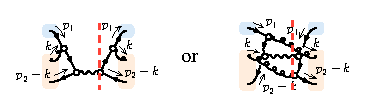
\includegraphics{thrown-out.pdf}
The remaining calculation consists of the bare parton model together with the \emph{minimal} set of multi-partonic contributions needed for IR finitess.
% Valentin PDF: page 3, annotation 351.
\valentin{I would rather say, the calculations presented in this paper, and at variance with those of your previous DIS paper, instead limit themselves to computing the minimal set\ldots{}}
%
%

%In this perspective, the $\overline{\text{MS}}$ PDFs $f_{\mathfrak{q}}^{\overline{\text{MS}}}$ re-absorb the contribution of all diagrams with many partons in the initial state, on top of the $\overline{\text{MS}}$ poles of the bare parton model cross-section.
%Another choice is to consider PDFs $f_{\mathfrak{q}}^{\text{LU}}$ that re-absorb the contribution of all and only the diagrams that are not strictly necessary to make the parton model finite.
%This leaves the computation of the parton model diagrams plus the minimal set of multi-partonic diagrams that make them IR finite, which is a gauge invariant subset of diagrams that independently factorises (as shown below).
%This is the LU scheme.

%{\color{red} $p_1^2,p_2^2$ diagrams}

%In the LU-scheme, the contribution of the additional diagrams may be packaged in an especially compact form.
%Take the $\overline{\text{MS}}$ parton model diagrams for DIS and collect them in a set $\Gamma_{\mathfrak{q}}$.
%Then, allow initial-state partons to have any virtuality, meaning they can be off-shell.
%Then at NLO and LP, the DIS partonic tensors read:
In the LU scheme, the contributing interference diagrams are packaged compactly (see, e.g., Fig.~\ref{fig:xbox-sum}).
Let $\Gamma_{\mathfrak{q}}$ denote the set of $\overline{\text{MS}}$ parton-model diagrams for DIS, and allow the initial-state partons to carry arbitrary virtualities.
At NLO and LP, the DIS partonic tensors read:
\begin{align}
\label{eq:disc_dis}
\left(W_{\mathfrak{q}}^{\text{LU},(1)}\right)^{\mu\nu}&=\sum_{G\in\Gamma_{\mathfrak{q}}}\int_0^{\Lambda^2} \frac{\mathrm{d}p^2}{8\pi^2}\frac{\text{disc}_{p^2}\text{disc}_{1-x}I_{\mathfrak{q} G}^{\mu\nu}}{\langle\mathfrak{q}\rangle}.
\end{align}
 The integrals $I_{\mathfrak{q} G}^{\mu\nu}$ are given as \emph{End Matter} material.
 The discontinuities in $p^2$ and $1-x$ account for the sums over initial- and final-state cuts, respectively.
 % The measure $\mathrm{d}p^2/(8\pi^2)=[\mathrm{d}p^2/(2\pi)](1/4\pi)$ contains one observable-normalisation factor.
 The operator $\text{disc}_{\tilde{s}}$ is both understood as a sum over Cutkosky cuts~\cite{Cutkosky:1960sp} in the $\tilde{s}$ channel (see Fig.~\ref{fig:xbox-sum}) or as the difference of the function it operates on evaluated at $\tilde{s}-i\varepsilon$ and $\tilde{s}+i\varepsilon$ (at LP, no subtleties such as those of Refs.~\cite{Bourjaily:2020wvq,Hannesdottir:2022xki,Abreu:2014cla,Abreu:2017enx} arise).
% Valentin PDF: page 3, annotation 353.
\valentin{is $\tilde{s}$ supposed to be a placeholder here? I would use capitalize X then.}
%
%

For hadronic collisions, the situation is analogous.
For DY, the NLO, LP cross-section reads:
\begin{align}
\label{eq:disc_dy}
\frac{\mathrm{d}\sigma_{\mathfrak{q}\mathfrak{q}'}^{\text{LU},(1)}}{\mathrm{d}q^2}&= \hspace{-0.2cm}\sum_{G\in\Gamma_{\mathfrak{q}\mathfrak{q}'}} \hspace{-0.15cm} \text{Re}\hspace{-0.05cm}\left[\prod_{i=1}^2\int_0^{\Lambda^2}\hspace{-0.1cm}\frac{\mathrm{d}p_i^2}{2\pi}\text{disc}_{p_i^2}\right] \! \frac{N_{ee}I_{ G}^{\mathfrak{q}\mathfrak{q}'}}{4\pi \hat{s}\langle\mathfrak{q}\rangle \langle\mathfrak{q}'\rangle},
\end{align}
{\color{red} $\pi^2$ term}
where the set $\Gamma_{\mathfrak{q}\mathfrak{q}'}$ is given in the \hyperref[sec:integrals_DIS_DY]{End Matter}.
There is one discontinuity for each incoming hadron. Since the discontinuity of a finite integral is still finite, we obtain that each individual graph summand is IR finite.
% Valentin PDF: page 3, annotation 355.
\valentin{This comment may not exactly fit here, but in general you could essentially recycle the original LU proof (i.e. ref [19]) to immediately argue that this sum of contributions is locally finite at any order. It may be nice to establish that connection more explicitly than it has been done alreayd in this text.}{\color{red} the original LU proof only works for final states}
%
%
%

\begin{figure*}[t]
  \centering
   \vspace{-0.5cm}
  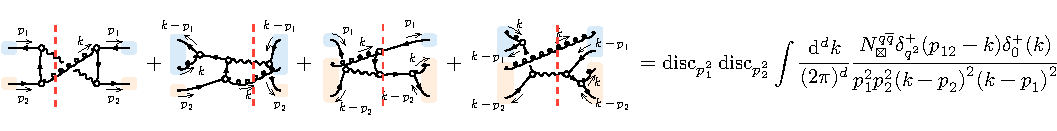
\includegraphics{xbox-sum.pdf}
  \vspace{-0.5cm}
  \caption{ \justifying Contribution of the $G=\timesbox$ cross-box diagram in the sum over $G\in \Gamma_{\mathfrak{q}\mathfrak{q}'}$ in \eqref{eq:disc_dy}, written as an (infrared-finite) discontinuity and as a sum of interference diagrams forming an infrared-finite class. The first diagram is the parton model's, while the additional ones form the minimal set of multi-partonic diagrams needed for its IR finiteness. Coloured shadings denote belonging to the $p_1$ (blue) jet or the $p_2$ (orange) jet, compatibly with the simplest-clustering criterion. The red line identifies the final-state cut. All initial- and final-state particles receive cut Feynman rules. On the right-hand side, we represent the integral $I_{\hspace{-0.075cm}\timesbox}^{\mathfrak{q}\mathfrak{q}'}$ as a vacuum graph embedding~\cite{Capatti:2025gqj}.
% Valentin PDF: page 4, annotation 397.
\valentin{This just one option, containing the collinear limits, but you should at least mention that one still needs to sum over all of them in principle (unless demonstratd to be non LP) and in particular remind again of the overlapping ones containing the soft, which will be unexpected/unfamiliar to some.}{\color{red} not sure what you mean}
%
%
% Valentin PDF v2: page 4, annotation 1222; updates original annotation 401.
\valentin{Did you not want to spell out explicitly in an equation what this I-cross-box is? You should refer to the corresponding equation there.
And I would take a chance in this caption that the very ability to rewrite the l.h.s from the r.h.s as prescribed in your earlier paper is what makes this entire procedure systematic.}{\color{red} I cross-box given in the end matter, that can be referenced. As far as second observation, not sure why that statement would be needed. The "systematicity" should be obvious from the statement, reiterating it without adding anything does not help.}
%
% Valentin PDF v2: page 4, annotation 1237.
\valentin{Why not keeping the flags on the vacuum cut?}
{\color{red} I'm agnostic}
%
% Valentin PDF v2: page 4, annotation 1377.
\valentin{Also you decayed the photon no? Maybe good to say that for clarity here you ommit the photon decay but you include it in your results later of course.}
{\color{red} the depicted relation is just true and does not rely on the decay of the photon. Results are consistent with photon decay as previously explained in the text}
%
%
  }
  \label{fig:xbox-sum}
  {\color{gray!50}\rule{0.8\linewidth}{0.6pt}}
  \phantom{g}\\[-0.3cm]
\end{figure*}

% The factor $1/(4\pi)$ is the single global observable-normalisation factor for the complete two-leg cluster.

We determine the universal scheme transformation of PDFs from the LU scheme to the $\overline{\text{MS}}$ scheme by standard Altarelli--Parisi (AP) techniques~\cite{Altarelli:1977zs}, adapted to our framework (see \emph{End Matter} material).
This also proves the factorisability of the minimal set of multi-partonic diagrams.
%
%
We introduce the \emph{splitting counterterms} $D_{\mathfrak{q}\mathfrak{q}'}$ by the relation $f_{\mathfrak{q}'}^{\overline{\text{MS}}}=D_{\mathfrak{q}'\mathfrak{q}}\otimes f_{\mathfrak{q}}^{\text{LU}}$:
\begin{equation}
f_{\mathfrak{q}'}^{\overline{\text{MS}}}(x;\mu^2)=\hspace{-0.15cm}\sum_{\mathfrak{q}\in\mathfrak{S}_1}\hspace{-0.05cm}\int_x^1 \hspace{-0.05cm}\frac{\mathrm{d}\xi}{\xi} D_{\mathfrak{q}'\mathfrak{q}}\hspace{-0.06cm}\left(\xi,\tfrac{\Lambda^2}{\mu^2}\right)f_{\mathfrak{q}}^{\text{LU}}\hspace{-0.06cm}\left(\tfrac{x}{\xi};\Lambda^2\right).
\end{equation}
% Valentin PDF: page 3, annotation 357.
\valentin{You should maybe formally define the convolution operator “circled\_cross” and then actually use it in your equations to shorten them.
Though looking at our usual definition (e.g. eq. 2.5 of \url{https://arxiv.org/pdf/2004.04752}) it’s a bit weird that you kept the lower bound of the convolving variable $\xi$ integrated over at 0 instead of x.
It’s abit weird as it means that your LU PDF should be dfined for an argument larger than one too at NLO?} {\color{red} fixed, as far as otimes symbol it's just above the equation}
%
%
The coupling expansion reads
\begin{equation}
D_{\mathfrak{q}\mathfrak{q}'}\left(\xi;\tfrac{\Lambda^2}{\mu^2}\right)=\sum_{n=0}^\infty \left(\frac{\alpha_s}{2\pi}\right)^{n} D_{\mathfrak{q}\mathfrak{q}'}^{(n)}\left(\xi;\tfrac{\Lambda^2}{\mu^2}\right),
\end{equation}
with $D_{\mathfrak{q}\mathfrak{q}'}^{(0)}=\delta_{\mathfrak{q}\mathfrak{q}'}\delta(1-\xi)$, and:
\begin{widetext}
\begin{align}
D_{\mathfrak{q}\mathfrak{q}'}^{(1)}(\xi)=
\left.
\sum_{\mathfrak{a}\in\mathfrak{S}_1}\int_0^1 \mathrm{d}\xi'\,
\frac{c_{\mathfrak{a}\mathfrak{q}'}}{\Gamma(1-\epsilon)}
\Bigg\{\left[\delta_{\mathfrak{q}\mathfrak{a}}\delta(\xi-\xi')
-\frac{\delta_{\mathfrak{q}\mathfrak{q}'}\delta(1-\xi)}2\right]
\frac{P_{\mathfrak{a}\mathfrak{q}'}^{(0)}(\xi')}{\epsilon}-\delta_{\mathfrak{q}\mathfrak{a}}\delta(\xi-\xi')b_\partial^{\mathfrak{a}\mathfrak{q}'}
\Bigg\}
\left(\frac{\Lambda^2\xi'\bar{\xi}'}
{e^{\gamma_E}\mu^2}\right)^{-\epsilon}
\right|_{\epsilon^0}. \label{eq:splitting_cts_nlo}
\end{align}

\end{widetext}

 Here, $\bar{\xi}'=1-\xi'$, $c_{qg}=T_F$, $c_{qq}=c_{gq}=C_F$ and $c_{gg}=C_A$.
 The function $P_{\mathfrak{q}\mathfrak{q}'}^{(0)}(\xi)$ is the leading-order AP splitting kernel in conventional dimensional regularisation, Eqs.~(32)-(35) of Ref.~\cite{Catani:1996pk}, stripped of colour factors, while $\big|_{\epsilon^0}$ stresses that the pole is discarded.
 The $\delta(\xi-\xi')$ pieces originate from the contribution with an additional QCD emission in the final state.
 Finally, $b_{\partial}^{qg}=1$, $b_{\partial}^{gq}=b_{\partial}^{qq}=1-\epsilon$, $b_{\partial}^{gg}=\tfrac{3(2\epsilon-3)}{4(1-\epsilon)}$ specify the Feynman-gauge boundary terms.
 Reverse Unitarity calculations require them, whereas Local Unitarity's are organised with $b_{\partial}^{\mathfrak{q}\mathfrak{q}'}=0$.
% Valentin PDF: page 3, annotation 359.
\valentin{I wonder how much the lower-bound change I suggest in Eq. 16 changes/simplifies things here\ldots{}}{\color{red} what should simplify? also want to remove this last ``Reverse Unitarity calculations require them, whereas Local Unitarity's are organised with $b_{\partial}^{\mathfrak{q}\mathfrak{q}'}=0$.'' sentence.}
%
%
%


\section{Reverse Unitarity computation}
\label{sec:reverse-unitarity}

We now compute the NLO DIS and DY cross-sections in the LU scheme using Reverse Unitarity, providing two benchmark tests of the correctness and universality of the splitting counterterms of Eq.~\eqref{eq:splitting_cts_nlo}.
In the following, we will use $f=f^{(0)}+\tfrac{\alpha_s}{2\pi}f^{(1)}+\mathcal{O}(\alpha_s^2)$ for the coupling expansion of the observable $f$.
%

\underline{\textbf{DIS}}: The structure functions are obtained from the partonic tensor by projection of the partonic tensors with the usual projectors, $F_{a\mathfrak{q}}=\mathrm{P}_a^{\mu\nu}(W_{\mathfrak{q}})_{\mu\nu}$.
We obtained in Ref.~\cite{Capatti:2025gqj} that, for a quark:
%
\begin{align}
\frac{F_{2q}^{\text{LU},(1)}}{e_q^2C_F x}
&=
\tilde{P}_{qq}^{(0)}(x)L_x-\frac{2\pi^2+3}{3}\delta(1-x)
\nonumber\\
&\hspace{1cm}
-\frac{6x^2-4x+1}{2(1-x)_+}
+\mathcal{O}\left(\tfrac{\Lambda^2}{q^2_{\text{h}}}\right),
\\
\frac{F_{Lq}^{\text{LU},(1)}}{e_q^2C_F x}
&= 2x+\mathcal{O}\left(\tfrac{\Lambda^2}{q^2_{\text{h}}}\right),
\end{align}
% Valentin PDF v2: page 4, annotation 1276.
\valentin{I know it’s standard, but I’d still spend a line defining the + distribution}{\color{red} We can reference a paper but I wouldn't spend a whole equation to explain it}
%
%
while for a gluon:
\begin{align}
\frac{F_{2g}^{\text{LU},(1)}}{2e_q^2 T_F x}&= \tilde{P}_{qg}^{(0)}(x)L_x+6x(1-x)-2+\mathcal{O}\left(\tfrac{\Lambda^2}{q^2_{\text{h}}}\right), \\
\frac{F_{Lg}^{\text{LU},(1)}}{2e_q^2 T_F x}&=4  x(1-x)+\mathcal{O}\left(\tfrac{\Lambda^2}{q^2_{\text{h}}}\right),
\end{align}
where $L_x=\log\left(\tfrac{Q^2}{\Lambda^2 x^2}\right)$ and $q_{\mathrm{h}}=\min(Q^2,(p+q)^2)$.
% Valentin PDF v2: page 4, annotation 1242.
\valentin{maybe write explicitly $q_h=\min(Q^2,(p+q)^2)$ then simply?}{\color{red} ok}
%
The function $\tilde{P}^{(0)}_{\mathfrak{q}\mathfrak{q}'}$ is the regularised Altarelli--Parisi splitting kernel, Eqs.~(C.6)-(C.9) of Ref.~\cite{Catani_1997}, stripped of colour factors.
The gluon structure functions account for a single quark flavour. 
%



The result is IR finite, owing to the KLN mechanism, and the scale evolution and longitudinal structure functions take the same form as in the $\overline{\text{MS}}$ parton model.
Hence, structure functions can be cast in the $\overline{\text{MS}}$ scheme by a scheme redefinition.
More precisely, we find that
\begin{equation}
F_{2\mathfrak{q}}^{\overline{\text{MS}}}=\sum_{\mathfrak{q}'\in\mathfrak{S}_1}D^{-1}_{\mathfrak{q}'\mathfrak{q}}\otimes F_{2\mathfrak{q}'}^{\text{LU}}+\mathcal{O}\left(\alpha_s^2,\tfrac{\Lambda^2}{q^2_{\text{h}}}\right),
\end{equation}
where the $D_{\mathfrak{q} \mathfrak{q}'}$ functions are precisely those of Eq.~\eqref{eq:splitting_cts_nlo}, with the Feynman-gauge boundary terms, and the $\overline{\text{MS}}$ result is given in Ref.~\cite{Bardeen:1978yd}.
%
%The Reverse Unitarity computation naturally captures boundary terms, and provides an independent cross-check of the direct splitting counter-term computation.


\underline{\textbf{DY}}: We can compute the NLO DY cross-section in the same formalism.
The Reverse Unitarity computation gives, using $q^2=z \hat{s}$,
%
\begin{align}
&\frac{\mathrm{d}\sigma_{q\bar{q}}^{\text{LU},(1)}}{\mathrm{d}q^2}= \frac{e_q^2 \alpha C_F}{3N_cq^2 \hat{s}}\! \Bigg[ 2\tilde{P}_{qq}^{(0)}(z)L_z -\delta(1-z)\!\nonumber \\
&+2(1+z^2)\! \left[\frac{\log(1\!-\! z)}{1\!-\!z}\right]_+ +2z-4 \Bigg] \!  +\mathcal{O}\left(\tfrac{\Lambda^2}{q^2_{\text{h}}}\right), \label{eq:qq_DY}\\
&\frac{\mathrm{d}\sigma_{qg}^{\text{LU},(1)}}{\mathrm{d}q^2}=\frac{e_q^2 \alpha T_F}{3N_cq^2 \hat{s}}\Bigg[
\tilde{P}_{qg}^{(0)}(z)\left(L_z+\log(1-z)\right) \nonumber
 \\
 &+\frac{-1+2z-3z^2}{2}\Bigg] +\mathcal{O}\left(\tfrac{\Lambda^2}{q^2_{\text{h}}}\right), \label{eq:qg_DY}
\end{align}
where $L_z=\log\left(\tfrac{\hat{s}}{\Lambda^2z}\right)$ and $q_{\mathrm{h}}=\min(\hat{s},q^2)$. 
Equations~\eqref{eq:qq_DY} and \eqref{eq:qg_DY} are related to the $\overline{\text{MS}}$ results~\cite{Altarelli:1979ub} by
\begin{align}
\hspace{-0.05cm}\frac{\mathrm{d}\sigma_{\mathfrak{q}\mathfrak{q}'}^{\overline{\text{MS}}}}{\mathrm{d}q^2}=\hspace{-0.3cm}\sum_{\mathfrak{q}_1,\mathfrak{q}_2\in\mathfrak{S}_1}\hspace{-0.3cm}D^{-1}_{\mathfrak{q}_1\mathfrak{q}}\otimes\frac{\mathrm{d}\sigma_{\mathfrak{q}_1\mathfrak{q}_2}^{\text{LU}}}{\mathrm{d}q^2}\otimes D^{-1}_{\mathfrak{q}_2\mathfrak{q}'}\hspace{-0.05cm}+\mathcal{O}\left(\alpha_s,\tfrac{\Lambda^2}{q^2_{\text{h}}}\right),
\end{align}
% Valentin PDF: page 4, annotation 399.
\valentin{For the sake of clarity, I would also explicit state the definition of that double-convolution notation; precedence rules would be a bit unclear otherwise.}{\color{red}It should be a symmetric commutative product}
%
%
which uses $D_{qq}$ and $D_{qg}$ as defined by Eq.~\eqref{eq:splitting_cts_nlo}.
%

These computations confirm that, at NLO, LU and $\overline{\text{MS}}$ cross-sections carry the same scale dependence and are related to each other by a universal scheme redefinition.

\section{Local Unitarity computation}
\label{sec:local-unitarity}

\begin{figure}[!tp]
\begin{minipage}{\columnwidth}
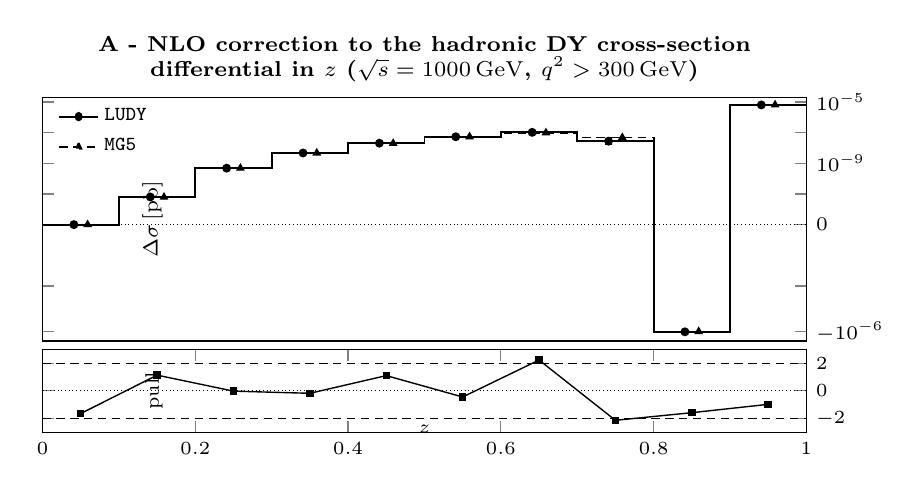
\begin{tikzpicture}
\begin{axis}[
  name=top,
  width=0.8\linewidth, height=88pt,
  scale only axis=true,
  xmin=0, xmax=1, ymin=-7.6, ymax=8.3,
  xtick=\empty,
  ytick={-7,-4,0,2,4,6,8},
  yticklabels={$-10^{-6}$,,$0$,,$10^{-9}$,,$10^{-5}$},
  ylabel={$\Delta\sigma\,[\mathrm{pb}]$},
  label style={font=\fontsize{7.4}{8.2}\selectfont},
  tick label style={font=\fontsize{6.95}{7.5}\selectfont},
  yticklabel pos=right,
  ylabel style={at={(axis description cs:0.17,0.5)},anchor=south},
  tick align=inside, tick style={line width=0.45pt},
  axis line style={line width=0.5pt},
  legend style={draw=none, fill=none, font=\fontsize{7.2}{8.0}\selectfont,
    at={(0.02,0.98)}, anchor=north west, cells={anchor=west},
    clip=false,
    inner sep=0pt, row sep=1.0pt},
  legend image post style={xscale=0.82},
  scaled ticks=false,
]
\addplot[forget plot, densely dotted, line width=0.35pt] coordinates {(0,0) (1,0)};
\addplot[forget plot, const plot, solid, line width=0.65pt, no markers] coordinates {
  (0,-1.0825609273e-07) (0.1,1.80636078274) (0.2,3.68698784682) (0.3,4.67784905565)
  (0.4,5.31675465815) (0.5,5.73659368841) (0.6,6.02551703723) (0.7,5.44886470855)
  (0.8,-6.99828623135) (0.9,7.81595078666) (1,7.81595078666)
};
\addlegendimage{solid,line width=0.65pt,mark=*,mark size=1.35pt}
\addlegendentry{\texttt{LUDY}}
\addplot[forget plot, only marks, mark=*, mark size=1.35pt,
  mark options={solid,line width=0.5pt},
  error bars/.cd, y dir=both, y explicit,
  error bar style={solid,line width=0.5pt}, error mark options={rotate=90,mark size=1.4pt,line width=0.5pt}
] table[x=x,y=y,y error plus=ep,y error minus=em,row sep=\\] {
x y ep em\\
0.041 -1.0825609273e-07 2.27343570652e-07 2.27343570652e-07\\
0.141 1.80636078274 0.00810868629094 0.00826296824384\\
0.241 3.68698784682 0.00492309845002 0.00497954646871\\
0.341 4.67784905565 0.00823607833342 0.0083952938262\\
0.441 5.31675465815 0.00744099487869 0.0075707110661\\
0.541 5.73659368841 0.00829014701607 0.00845148036611\\
0.641 6.02551703723 0.0109602517208 0.011244031816\\
0.741 5.44886470855 0.126880367248 0.180000757748\\
0.841 -6.99828623135 0.0137818203332 0.0133578890847\\
0.941 7.81595078666 0.00410287647731 0.00414200723387\\
};
\addplot[forget plot, const plot, densely dashed, line width=0.65pt, no markers] coordinates {
  (0,3.75236795494e-06) (0.1,1.79326940422) (0.2,3.68710984322) (0.3,4.67935942987)
  (0.4,5.30823156739) (0.5,5.74036460039) (0.6,5.99966763758) (0.7,5.68630817528)
  (0.8,-6.97623986543) (0.9,7.81999602799) (1,7.81999602799)
};
\addlegendimage{densely dashed,line width=0.65pt,mark=triangle*,mark size=1.35pt}
\addlegendentry{\texttt{MG5}}
\addplot[forget plot, only marks, mark=triangle*, mark size=1.35pt,
  mark options={solid,line width=0.5pt},
  error bars/.cd, y dir=both, y explicit,
  error bar style={solid,line width=0.5pt}, error mark options={rotate=90,mark size=1.4pt,line width=0.5pt}
] table[x=x,y=y,y error plus=ep,y error minus=em,row sep=\\] {
x y ep em\\
0.059 3.75236795494e-06 2.34504582056e-06 2.34504582056e-06\\
0.159 1.79326940422 0.00804724754357 0.00819917842147\\
0.259 3.68710984322 0.00316829733376 0.00319158089559\\
0.359 4.67935942987 0.00202991908187 0.00203945162144\\
0.459 5.30823156739 0.00155242901133 0.00155799823762\\
0.559 5.74036460039 0.001608182016 0.00161415921559\\
0.659 5.99966763758 0.00201370813004 0.0020230886716\\
0.759 5.68630817528 0.0100499473373 0.0102880321129\\
0.859 -6.97623986543 0.00135389618765 0.00134968858249\\
0.959 7.81999602799 0.000608724131456 0.00060957854072\\
};
% Title above histogram
\node[
  anchor=south,
  align=center,
  font=\fontsize{7.8}{8.8}\selectfont\bfseries
] at (axis description cs:0.5,1.025)
{A - NLO correction to the hadronic DY cross-section \\ differential in $z$ 
($\sqrt{s}=1000\,\mathrm{GeV}$, $q^2>300\,\mathrm{GeV}$)};
% Horizontal rule above title
\end{axis}
\begin{axis}[
  at={(top.south west)}, anchor=north west, yshift=-3pt,
  width=0.8\linewidth, height=30pt,
  scale only axis=true,
  xmin=0, xmax=1, ymin=-3.0, ymax=3.0,
  xtick={0,0.2,0.4,0.6,0.8,1},
  xticklabels={$0$,$0.2$,$0.4$,$0.6$,$0.8$,$1$},
  ytick={-2,0,2},
  xlabel={$z$}, ylabel={pull},
  label style={font=\fontsize{7.05}{7.7}\selectfont},
  tick label style={font=\fontsize{6.7}{7.25}\selectfont},
  xlabel style={at={(axis description cs:0.5,0.2)},anchor=north},
  ylabel style={at={(axis description cs:0.17,0.5)},anchor=south},
  tick align=inside, tick style={line width=0.45pt},
  yticklabel pos=right,
  axis line style={line width=0.5pt},
  clip=true,
]
\addplot[forget plot, densely dotted, line width=0.35pt] coordinates {(0,0) (1,0)};
\addplot[forget plot, densely dashed, line width=0.35pt] coordinates {(0,2) (1,2)};
\addplot[forget plot, densely dashed, line width=0.35pt] coordinates {(0,-2) (1,-2)};
\addplot[solid, line width=0.5pt, mark=square*, mark size=1.1pt] coordinates {
  (0.05,-1.639) (0.15,1.135) (0.25,-0.021) (0.35,-0.177) (0.45,1.102)
  (0.55,-0.444) (0.65,2.228) (0.75,-2.129) (0.85,-1.578) (0.95,-0.975)
};

\end{axis}
\end{tikzpicture}
\end{minipage}
\phantom{g}\\[0.1cm]
\begin{minipage}{0.45\textwidth}
\begin{minipage}{1\textwidth}
{\fontsize{7.8}{8.8}\selectfont\bfseries
B - NLO corrections to total $\mathfrak{q}\mathfrak{q}'\rightarrow t \bar{t}$ cross-section
\par}
\phantom{}\\[-0.2cm]
\begin{tabular}{
@{\hspace{5pt}}
l@{\hspace{10pt}}
l@{\hspace{10pt}}
>{\columncolor{ludybg}[4pt][4pt]}l@{\hspace{10pt}}
>{\columncolor{refbg}[4pt][4pt]}l@{\hspace{8pt}}
r@{\hspace{5pt}}
}
\topblackrule
\scalebox{0.9}{$\sqrt{\hat s}$ [$\scalebox{0.8}{$\text{GeV}$}$]}
& \scalebox{0.9}{$\mathfrak{q}\mathfrak{q}'$}
& \scalebox{0.9}{\texttt{LUDY} [$\scalebox{0.8}{$10^{-9}\,\text{GeV}^{-2}$}$]}
& \scalebox{0.9}{\cite{Czakon:2008ii} [$\scalebox{0.8}{$10^{-9}\,\text{GeV}^{-2}$}$]}
& \scalebox{0.9}{pull} \\
\midblackrule

\multirow{3}{*}{$400$}
 & $q\bar q$ & $-8.650(27)$
 & $-8.694003$ & $+1.65$ \\
 & $qg$ & $-0.40523(58)$
 & $-0.405162$ & $-0.11$ \\
 & $gg$ & $\phantom{-}8.957(87)$
 & $\phantom{-}9.048046$ & $-1.05$ \\
\midblackrule

\multirow{3}{*}{$1000$}
 & $q\bar q$ & $-3.8161(98)$
 & $-3.799312$ & $-1.71$ \\
 & $qg$ & $\phantom{-}6.742(12)$
 & $\phantom{-}6.732486$ & $+0.73$ \\
 & $gg$ & $\phantom{-}23.12(25)$
 & $\phantom{-}22.98039$ & $+0.55$ \\
\midblackrule

\multirow{3}{*}{$2000$}
 & $q\bar q$ & $\phantom{-}0.0169(86)$
 & $\phantom{-}0.007436$ & $+1.10$ \\
 & $qg$ & $\phantom{-}14.219(37)$
 & $\phantom{-}14.30716$ & $-2.35$ \\
 & $gg$ & $\phantom{-}60.75(38)$
 & $\phantom{-}61.20165$ & $-1.20$ \\
\bottomblackrule
\end{tabular}
\end{minipage}
\end{minipage}
\begin{minipage}{0.45\textwidth}
\begin{minipage}{1\textwidth}
{\fontsize{7.8}{8.8}\selectfont\bfseries
C - NLO corrections to total $PP\rightarrow t \bar{t}$ cross-section
\par}
\phantom{g}\\[-0.25cm]
\begin{tabular}{
@{\hspace{5pt}}
l@{\hspace{10pt}}
>{\columncolor{ludybg}[4pt][4pt]}l@{\hspace{12pt}}
>{\columncolor{mgfivebg}[4pt][4pt]}l@{\hspace{12pt}}
l@{\hspace{5pt}}
}
\topblackrule
\scalebox{0.9}{$\sqrt{s}$ [\scalebox{0.8}{$\text{GeV}$}]}
& \scalebox{0.9}{\texttt{LUDY} [\scalebox{0.8}{$\mathrm{pb}$}]}
& \scalebox{0.9}{\texttt{MG5} [\scalebox{0.8}{$\mathrm{pb}$}]}
& \scalebox{0.9}{pull} \\
\midblackrule
$400$
& $1.0553(40)\!\cdot\!10^{-9}$
& $1.0498(71)\!\cdot\!10^{-9}$
& $+1.34$ \\

$1000$
& $4.408(53)\!\cdot\!10^{-3}$
& $4.4288(58)\!\cdot\!10^{-3}$
& $-0.40$ \\

$1500$
& $6.00(10)\!\cdot\!10^{-2}$
& $5.999(10)\!\cdot\!10^{-2}$
& $+0.03$ \\

$2000$
& $2.521(92)\!\cdot\!10^{-1}$
& $2.5239(50)\!\cdot\!10^{-1}$
& $-0.03$ \\
\bottomblackrule
\end{tabular}
\end{minipage}
\end{minipage}
\begin{minipage}{0.45\textwidth}
\begin{minipage}{1\textwidth}
{\fontsize{7.8}{8.8}\selectfont\bfseries
Parameters
\par}
\phantom{g}\\[-0.25cm]
\begingroup
\fontsize{7.4}{8.2}\selectfont
\begin{tabular}{
|@{\hspace{5pt}}
l@{\hspace{7pt}}l
@{\hspace{7pt}}|@{\hspace{7pt}}
l@{\hspace{7pt}}l
@{\hspace{5pt}}|
}
\hline
\rule{0pt}{2.8ex}$\alpha_s$ & $0.118$
& $\alpha^{-1}$ & $132.507$ \\

$\mu=\Lambda$ & $91.118\,\mathrm{GeV}$
& $m_t$ & $173\,\mathrm{GeV}$ \\

$f_{\mathfrak q}$ &
\texttt{PDF4LHC21\_40} (ID $93100$)~\cite{PDF4LHCWorkingGroup:2022cjn}
& $e_q$ & $e/3$ \\[1.5pt]
\hline
\end{tabular}
\endgroup

\end{minipage}
\end{minipage}

\caption{\justifying Results for the Drell--Yan and $t\bar{t}$-production processes, using Local Unitarity (\texttt{LUDY}), converted to the $\overline{\text{MS}}$ scheme. Results for \textbf{A} are obtained with 24M points for the full histogram and 2M refinements for the first three bins, with evaluation time at $\sim$4ms. Results for \textbf{B} are obtained with 100M points per channel and $\sqrt{\hat{s}}$, 400M for $gg$, 400GeV, with typical evaluation times at $\sim$1-10ms, depending on the channel. Results for \textbf{C} are obtained with 200M points per $\sqrt{s}$, 100M for $\sqrt{s}=400$GeV, with typical evaluation times at $\sim$20ms. See \emph{End Matter} for a discussion of numerical performance.}
{\color{gray!50}\rule{0.8\linewidth}{0.6pt}}
\label{fig:results}
\phantom{g}\\[-0.5cm]
\end{figure}
%


We exploit the IR finiteness of hadronic cross-sections in the $\text{LU}$ scheme to compute them in $d=4$ using Monte Carlo methods.
The finite hard shifts generated by $D^{-1}_{\mathfrak{q}\mathfrak{q}'}$ are added to the LU result to match the $\overline{\text{MS}}$ scheme.
%
% , equivalently minus the finite parts of eq.~\eqref{eq:splitting_cts_nlo},
For DY, one computes the bin contribution
\begin{equation}
%\Delta_{ab}\sigma_{\mathfrak{q}\mathfrak{q}'}^{\text{LU},(1)}=
\int_a^b \mathrm{d}z\frac{\mathrm{d}\sigma_{\mathfrak{q}\mathfrak{q}'}^{\text{LU},(1)}}{\mathrm{d}z}=\sum_{G\in\Gamma_{\mathfrak{q}\mathfrak{q}'}}\frac{N_{ee}\Delta_{ab}^G}{4\pi \langle\mathfrak{q}\rangle \langle\mathfrak{q}'\rangle},
\end{equation}
where
\begin{equation}
\Delta_{ab}^G=\!\int_a^b \mathrm{d}z\left[\prod_{i=1}^2\int_0^{\Lambda^2}\frac{\mathrm{d}p_i^2}{2\pi}\text{disc}_{p_i^2}\right] \! I_{ G}^{\mathfrak{q}\mathfrak{q}'}.
\end{equation}
Writing discontinuities in terms of cut Feynman diagrams, and performing the residual (if any) energy integrations using the Loop Tree Duality~\cite{Catani:2008xa,Bierenbaum:2010cy,PhysRevLett.122.111603,Capatti:2019ypt} (or equivalent~\cite{JesusAguilera-Verdugo:2020fsn,Capatti:2020ytd,Capatti:2022mly,bobadilla2021lottylooptreeduality}), we obtain the general form:
\begin{equation}
\Delta_{ab}^G=\! \int_{a}^b \mathrm{d}z\int\mathrm{d}\Pi_k \sum_{C_\sigma\in\mathcal{C}_G} \frac{\prod_{j\in C} \delta^{\sigma_j}(D_j)}{\prod_{i\in E\setminus C }D_i}N_{\mathfrak{q}\mathfrak{q}'}^G,
\end{equation}
where
\begin{equation}
\label{eq:measure_pik}
\mathrm{d}\Pi_k=\left[\prod_{i=1}^2\frac{\mathrm{d}p_i^2}{2\pi}\Theta(\Lambda^2-p_i^2)\right]\frac{\mathrm{d}^4 k}{(2\pi)^4},
\end{equation}
and $N_{\mathfrak{q}\mathfrak{q}'}$ is the numerator, a polynomial in $k, p_1, p_2$, $D_j=q_j^2-m_j^2$.
% Valentin PDF v2: page 5, annotation 1296.
\valentin{In the Feynman gauge only (prolly good to stress). Otherwise a rational polynomial.}
%
% Valentin PDF v2: page 5, annotation 1471.
\valentin{Since this establishes clearly you’re in the feynman gauge you \emph{MUST} really add the ghost to your enumeration of possible initial-state earlier.}{\color{red} external gluons are transverse, internal ones are in the feynman gauge. No need for external ghosts. But feynman gauge can be stressed, which I do in end matter.}
%
%
%
The sum runs over all tuples $C_\sigma=(\sigma,C)\in\mathcal{C}_G$ of cut sets $C\subset E$ and signs $\sigma\in\{\pm 1\}^{|C|}$, compatible with the energy integration and the expansion of the discontinuity in terms of cut diagrams.
Each contribution now has, for DY, $|C|=4$ (for $t\bar{t}$, $|C|=5$).
% Valentin PDF v2: page 5, annotation 1301.
\valentin{I would really here stress again the general embedding construction of your previous paper, and also refer to Fig.1 again.}
%
Whenever a cut crosses a repeated propagator, the generalised cutting rule must be used~\cite{Capatti:2022tit}.

The LP contribution is obtained by an asymptotic expansion in $\Lambda^2$, using the expansion-by-regions method~\cite{Chetyrkin:1988zz,Gorishnii:1989dd,etde_6475136,Beneke:1997zp,Jantzen:2011nz,Gardi:2022khw}.
We find that all the regions are of hard, (anti-)collinear, soft, soft-(anti-)collinear~\footnote{We refer to ultrasoft regions as soft-(anti-)collinear since the transverse directions scale to zero faster than the longitudinal directions.} type:
\begin{equation}
\Delta_{ab}^G=\! \int_{a}^b \mathrm{d}z\int\mathrm{d}\Pi_k \sum_{C_\sigma, R} \frac{\prod_{j\in C} \delta^{\sigma_j}(D_j^R)}{\prod_{i\in E\setminus C }D_i^R}N_{\mathfrak{q}\mathfrak{q}'}^{G,R},
\end{equation}
where $D_i^R$ and $N_{\mathfrak{q}\mathfrak{q}'}^{G,R}$ are the propagators and numerator approximated in the region $R$.
The expansion-by-regions of the cut diagrams maps to that of the uncut contribution $I_{ G}^{\mathfrak{q}\mathfrak{q}'}$.
The bare parton model only selects the hard contribution of $I_{ G}^{\mathfrak{q}\mathfrak{q}'}$. 
% Valentin PDF v2: page 5, annotation 1307.
\valentin{Very important to stress that this is in principle NOT NEEDED.
Indeed, \emph{NOT DOING} so does not break IR finiteness and is STILL verifies Eq. (23), just with different subleading term. This is at variance with the traditional method where one could only obtain IR finiteness when working out resummation.
In other terms, you only need to do this here because you want to precisely identify and verify the universal scheme conversion term.}{\color{red} ok if there's a short way to say that.}
%
%
%

We then introduce an auxiliary scaling variable $t$ in line with Soper's trick~\cite{Soper_2000,Capatti:2020xjc}, rescaling $z\rightarrow t^2 z$ and $\mathbf{k}\rightarrow t \mathbf{k}$, and finally solve the four Dirac delta functions in $p_1^2,p_2^2,k^0,t$.
% Valentin PDF v2: page 5, annotation 1313.
\valentin{Why is a radial scaling centered at the coordinate origin always a calid causal flow in this case?}{\color{red} it just is, I don't think I want to spend time on these details in this paper}
%
%
That gives an integrand that is locally free of infrared singularities and can be directly fed to a Monte Carlo integrator.
%We provide a detailed example of this integrand manipulation as \emph{End Matter} material.
Finally, we should note that ultraviolet singularities are renormalised locally by the BPHZ-based~\cite{BogoliubowParasiuk1957,Zimmermann1969,Hepp1966} procedure of Ref.~\cite{Capatti:2022tit}, and acquire dependence on a UV renormalisation scale $\mu$, which can be varied independently from the factorisation scale $\Lambda$.
% Valentin PDF v2: page 5, annotation 1324.
\valentin{on THE renormalization scale $\mu_r$, i.e. include the \texttt{\_r} here I’d say}
%
Thresholds of loop diagrams are subtracted by the counterterm procedure of Ref.~\cite{Kermanschah:2021wbk}, being careful to correctly zero their contribution close to soft singularities (see fig.~\ref{fig:triangle_region}).
% Valentin PDF v2: page 5, annotation 1334.
\valentin{“zero a contribution” is weird, I’d say “regularize” and also it’d be honest to say that this is a hard problem with no general solution yet.
Also mention Fig. 4 there!}
{\color{red} no it's zeroed not regularised. ok with fig.4 references}
%
% Valentin PDF v2: page 10, annotation 1501; concerns Fig. 4's counterterm.
\valentin{Why not writing explicitly the functional form of your threshold CTs?
I think you really should.}
{\color{red} no space and technical, that fits to a longer companion paper}
%
%





We report in Fig.~\ref{fig:results} Monte Carlo results for the DY (differential in $z$) and $pp\rightarrow t \bar{t}$ (inclusive) hadronic cross-sections at NLO, using our path-finder code \texttt{LUDY}.
% Valentin PDF v2: page 5, annotation 1339.
\valentin{It’d be nice to shoutout gammaloop and symbolica (e.g. the website) in main text already?}{\color{red} ok if it can be done in short space}
%
% Figure-specific remarks stay beside its discussion so the composite float fits.
% Valentin PDF v2: page 5, annotation 1345; Fig. 2, panel A.
\valentin{Add rel. error subplot, not just pull?}
{\color{red} also space issue, would choose one of the two}
%
% Valentin PDF v2: page 5, annotation 1356; Fig. 2, panel A.
\valentin{x-axis label}
{\color{red} somehow layout screwed, not sure why}
%
% Valentin PDF v2: page 5, annotation 1361; Fig. 2, panel A.
\valentin{$\hat{s}$? not $s$?
Also $>300$ GeV? or $\mathrm{GeV}^2$? You seem to have a datapoint close to $z=0.05$ or so which seems lower if not squared.}
{\color{red} caption is correct, it's $\hat{s}$}
%
%
% Valentin PDF v2: page 5, annotation 1371; Fig. 2, panel A.
\valentin{Also is $q^2$ the off-shellness of your photon?
If so it’s not true that $q^2=zs$ for the real-emission diagram no? This is confusing.}
{\color{red} caption is correct for both virtual (z=1) and real (0<z<1)}
%
% Valentin PDF v2: page 5, annotation 1398; Fig. 2, panel A legend.
\valentin{Citation}
%
% Valentin PDF v2: page 5, annotation 1419; Fig. 2, panel C.
\valentin{Big tension here, pull values incorrect. Verify them all!}
{\color{red} to reverify, but they looked correct}
%
%
% Valentin PDF v2: page 5, annotation 1410; Fig. 2, parameter table.
\valentin{$\alpha_s(\mu_r^2=m_Z^2)$}
{\color{red} ok with a minor change}
%
%
% Valentin PDF v2: page 5, annotation 1409; Fig. 2, parameter table.
\valentin{I would not use Lambda but really the traditional $\mu_f$ here.}
{\color{red} $\Lambda^2$ would force the reader to understand what's happening in my opinion}
%
%
We use one $d$-quark flavour, $q=d$.
Agreement with the $\overline{\text{MS}}$ cross-sections for all partonic channels is achieved after the scheme conversion Eq.~\eqref{eq:splitting_cts_nlo} (with $b_\partial^{\mathfrak{q}\mathfrak{q}'}=0$), both at the partonic~\cite{Altarelli:1979ub,Czakon:2008ii, 1988NuPhB.303..607N} and hadronic~\cite{Alwall:2014hca} level, confirming that $D_{gg}$ and $D_{qg}$ are also correct.
The $\texttt{MG5aMC}$ result required the introduction of the decoupling-scheme counterterm to obtain agreement.
% Valentin PDF v2: page 5, annotation 1388.
\valentin{Citation and version info for MG.
Also refer to it as \texttt{MG5aMC}}
{\color{red} citation just above; as far as version i'll check}
%
%


\section{Outlook}
%

We successfully constructed hadronic cross-sections in terms of partonic cross-sections with an arbitrary number of initial-state partons, that are infrared finite without the need of PDF renormalisation, and compatibly with collinear factorisation.
% Valentin PDF v2: page 6, annotation 1438.
\valentin{to me “compatible the KLN theorem” sounds weak.
The real important corollary of this is that you did it in way that you get an IR-finite fixed-order differential cross-section without relying on factorization/resummation, though, as you show, compatible with it of course.
This is the more striking feature to highlight here in my opinion.}
{\color{red} ok}
%
We have done so by analytic and Monte Carlo computations of three paradigmatic QCD cross-sections, developing in the process a \emph{fully local} approach to the calculation.
% Valentin PDF v2: page 6, annotation 1433; targets “paradigmatic”.
\valentin{I don’t like the world} {\color{red} ?}
%
%
Two future research directions arise in particular: 
%if this organisation remains computationally viable at higher perturbative orders and if its $\Lambda^2$ expansion provides a true description of power corrections.
% Valentin PDF v2: page 6, annotation 1427.
\valentin{double iterated colon sentence; weird.}
{\color{red} ok}
%
%

\begin{itemize}
\item[\textit{i}] \textit{Generalisation to NNLO LP}: extending the formalism at NNLO would allow us to compute hadronic cross-sections entirely by Monte Carlo methods, including loop integrals, in momentum space.
This program is core to both the Local Unitarity and the ETHZ-Stony Brook subtraction frameworks~\cite{Anastasiou:2018rib,Anastasiou:2020sdt,Anastasiou:2022eym,Anastasiou:2024xvk,Anastasiou:2026kpm,Capatti:2019ypt,Capatti:2019edf,Kermanschah:2021wbk,Kermanschah:2024utt,Kermanschah:2025wlo}, and has the potential to overcome current computational bottlenecks in the production of precise fixed-order predictions.
%

\item[\textit{ii}] \textit{Power corrections} The $\Lambda^2$ expansion in our formalism is controlled, and the subleading-power contributions of any cross-section can be written in terms of cut Feynman integrals.
% Valentin PDF v2: page 6, annotation 1444.
\valentin{“in principle” is weird, I would say “formally” or smtg like this}
{\color{red} ok}
%
Importantly, the method is gauge invariant by construction.
% Valentin PDF v2: page 6, annotation 1451.
\valentin{I don’t care why this makes sense to highlight here?}
{\color{red} because massified gluon approaches are not}
%
%
Furthermore, KLN-based approaches have been used to probe linear power corrections~\cite{Akhoury_1996,Akhoury:1995sp}.
A natural extension is to compute subleading-power corrections for the DIS process, where an Operator Product Expansion is available and understood at subleading twist~\cite{JAFFE1981467,Ellis:1982cd}.
Beyond DIS, comparisons with operator~\cite{Qiu:1990xxa,Feige2017SubleadingFactorization,Moult:2018jjd,Moult2017SubleadingBasis,Moult2018SubleadingResummation,Moult2019RadiativeFunctions,Beneke2018SubleadingNJet,Beneke2019NLPDrellYan,Beneke2020ThresholdFactorization}, dispersive~\cite{Dokshitzer1998Milan,DokshitzerMarchesiniWebber1996Dispersive,DokshitzerWebber1995PowerCorrections} and massified-gluon/renormalon~\cite{Korchemsky_1995,NasonSeymour1995Renormalons,BenekeBraun1995DrellYan,FerrarioRavasio2019Renormalons,Caola:2021kzt,Caola:2022vea} approaches can be considered.
% Valentin PDF v2: page 6, annotation 1477.
\valentin{“should” is weird here.
I’d say, “can be considered.” perhaps.}
{\color{red} ok}
%

\end{itemize}

Finally, the infrared interplay between the multi-partonic contributions and the parton-model diagrams could be a basis for studies of factorisation and factor\-isation-breaking~\cite{Collins:2007nk,Rogers:2010dm,Catani:2011st,Forshaw:2012bi,Gaunt:2014ska,Zeng:2015iba,Rothstein:2016bsq,Schwartz:2017nmr,Becher:2023lmy,Becher:2024vdk}, especially due to our inclusion of spectator particles.
Our framework is uniquely positioned to simultaneously attack these questions.
% Valentin PDF v2: page 6, annotation 1483.
\valentin{“simultaneously” is weird, I’d say “attack these questions within one unifying framework”.}
%
%


\begin{acknowledgments}
\paragraph{Acknowledgements} We are grateful to Valentin Hirschi for his invaluable support and input throughout the development of this work.
We are also thankful to Michael Ruf for several discussions.
The work of the authors is supported by the Swiss National Science Foundation under grant agreement PCEFP2\_203335.
The work of Z.C. is also supported by the European Union under the Marie Skłodowska-Curie Actions, grant agreement No. 101271880. \textbf{LLM use}: the authors made extensive use of the GPT-5 and GPT-6 models in the development of this work. Both authors hold ChatGPT Pro subscriptions. All analytical calculations reported in the paper were performed at least once by a human without AI assistance. The \texttt{LUDY} code was developed with substantial AI assistance, particularly after the release of GPT-5.4. The manuscript itself was written by the authors; AI tools were used only in an editorial capacity.
%
%
 
\end{acknowledgments}

\bibliography{apssamp}

\section{End matter}
%
\subsection{List of integrals for DIS and DY}
\label{sec:integrals_DIS_DY}

\begin{figure}
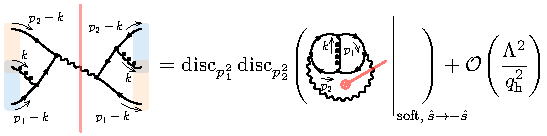
\includegraphics[width=\linewidth]{soft-triangle.pdf}
\caption{\justifying An example of a non-trivial identification, at leading power, of cut diagrams with discontinuities. In this case, the interference diagram where the gluon belongs to both jets at the same time is equated to the double discontinuity of the sum of the soft and soft-collinear regions of the integral $I_{\triangle}^{q\bar{q}}$, represented as an embedding.{\color{red} reverse p1 arrow}
%
}
\label{fig:triangle_soft}
{\color{gray!50}\rule{0.8\linewidth}{0.6pt}}
\phantom{g}\\[-0.3cm]
\end{figure}

Here we provide a list of the integrals appearing in Eq.~\eqref{eq:disc_dis} and Eq.~\eqref{eq:disc_dy}.
% Valentin PDF v2: page 9, annotation 1493; targets the End Matter heading.
\valentin{How about Appendices like everybody else :P}{\color{red} end matter standard for PRL}
%
As mentioned, at LP, their discontinuities can be computed either by computing the integrals and then using the usual definition of discontinuity, or by writing the discontinuity as a sum over cut Feynman integrals (corresponding to the original interference diagrams). The equivalence between the two definitions is non-trivial, but can be shown, using the expansion-by-regions method (see, e.g., Fig.~\ref{fig:triangle_soft}), or by direct computation~\cite{Capatti:2025gqj}.   
%


\begin{figure}[!tp]
\scalebox{0.6}{
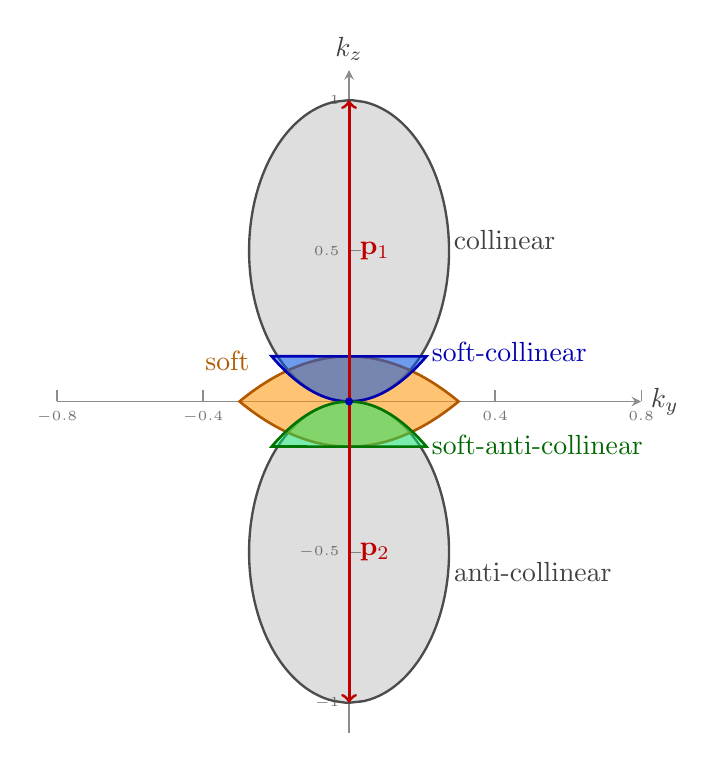
\begin{tikzpicture}
\begin{axis}[
  width=9cm,
  height=10cm,
  xmin=-0.8, xmax=0.8,
  ymin=-1.1, ymax=1.1,
  xtick distance=0.4,
  tick label style={black!55, font=\tiny},
  tick style={black!45, line width=0.45pt},
  axis lines=middle,
  axis line style={black!45, line width=0.55pt},
  xlabel={$k_y$},
  ylabel={$k_z$},
  xlabel style={anchor=west, text=black!75},
  ylabel style={anchor=south, text=black!75},
  tick align=inside,
  samples=160,
  clip=true,
]

% RegionPlot: y^2 + 0.3 z (1+z) < 0
% shifted upward by 1: plotted at vertical coordinate z+1
\path[
  fill=black!65,
  fill opacity=0.20,
  draw=black!70,
  line width=0.85pt
]
  plot[domain=-1:0, samples=180, variable=\z]
    (axis cs:{sqrt(-0.3*\z*(1+\z))},{\z+1})
  -- plot[domain=0:-1, samples=180, variable=\z]
    (axis cs:{-sqrt(-0.3*\z*(1+\z))},{\z+1})
  -- cycle;

\path[
  fill=black!65,
  fill opacity=0.20,
  draw=black!70,
  line width=0.85pt
]
  plot[domain=0:1, samples=180, variable=\z]
    (axis cs:{sqrt(0.3*\z*(1-\z))},{\z-1})
  -- plot[domain=1:0, samples=180, variable=\z]
    (axis cs:{-sqrt(0.3*\z*(1-\z))},{\z-1})
  -- cycle;

% softCollplot region 2
\path[
  fill=orange!85!yellow,
  fill opacity=0.55,
  draw=orange!70!black,
  line width=0.95pt
]
  plot[domain=-1.15:-1, samples=100, variable=\z]
    (axis cs:{sqrt(0.6*(\z+1.15))},{\z+1})
  -- plot[domain=-1:-0.85, samples=100, variable=\z]
    (axis cs:{sqrt(0.6*(-\z-0.85))},{\z+1})
  -- plot[domain=-0.85:-1, samples=100, variable=\z]
    (axis cs:{-sqrt(0.6*(-\z-0.85))},{\z+1})
  -- plot[domain=-1:-1.15, samples=100, variable=\z]
    (axis cs:{-sqrt(0.6*(\z+1.15))},{\z+1})
  -- cycle;

% softCollplot region 1
\path[
  fill=blue!65!cyan,
  fill opacity=0.50,
  draw=blue!70!black,
  line width=0.95pt
]
  plot[domain=-1:-0.85, samples=100, variable=\z]
    (axis cs:{sqrt(0.3*(\z+1))},{\z+1})
  -- plot[domain=-0.85:-1, samples=100, variable=\z]
    (axis cs:{-sqrt(0.3*(\z+1))},{\z+1})
  -- cycle;

% softCollplot2
\path[
  fill=green!55!cyan,
  fill opacity=0.45,
  draw=green!45!black,
  line width=0.95pt
]
  plot[domain=-0.15:0, samples=100, variable=\z]
    (axis cs:{sqrt(-0.3*\z)},{\z})
  -- plot[domain=0:-0.15, samples=100, variable=\z]
    (axis cs:{-sqrt(-0.3*\z)},{\z})
  -- cycle;

% Red arrows
\addplot[
  red!75!black,
  line width=1.1pt,
  ->
] coordinates {(0,0) (0,1)}
  node[midway, right, text=red!75!black] {$\mathbf{p}_1$};

\addplot[
  red!75!black,
  line width=1.1pt,
  ->
] coordinates {(0,0) (0,-1)}
  node[midway, right, text=red!75!black] {$\mathbf{p}_2$};

% Labels
\node[
  below right,
  text=orange!70!black
] at (axis cs:-0.42,0.2) {soft};

\node[
  below right,
  text=blue!70!black
] at (axis cs:0.2,0.23) {soft-collinear};

\node[
  below right,
  text=green!40!black
] at (axis cs:0.2,-0.08) {soft-anti-collinear};

\node[
  below right,
  text=black!75
] at (axis cs:0.26,0.6) {collinear};

\node[
  below right,
  text=black!75
] at (axis cs:0.26,-0.5) {anti-collinear};

% Origin marker
\addplot[
  only marks,
  mark=*,
  mark size=1.25pt,
  blue!70!black
] coordinates {(0,0)};

\end{axis}
\end{tikzpicture}



}
\caption{\justifying For the infrared-finite class of the DY process containing the virtual triangle diagram, the cancelling bulk singularities are located at the soft origin point, on the (anti-)collinear segment (in red), and on the black threshold circle. The parton-model diagram contributes with a hard region, and is non-zero everywhere in the loop momentum ($k$) space. Each additional multi-partonic cut has support only in compact regions (the shaded ``collinear'', ``soft-collinear'', and ``soft'' regions), due to the theta functions in Eq.~\eqref{eq:measure_pik}, while the threshold counterterm has support in the striped region, designed to exclude the collinear segment and so that the principal value of the counterterm is zero.
In the tiny sliver obtained by subtracting the collinear region from the soft-collinear region, the integrand is unbounded. The sliver narrows toward the soft point, yielding integrable behaviour.}
%
{\color{gray!50}\rule{0.8\linewidth}{0.6pt}}
\phantom{g}\\[-0.3cm]
\label{fig:triangle_region}
\end{figure}

\textbf{DIS:} For DIS, we have $\Gamma_{q}=\{\triangle,\Box,\bigcirc,\text{lsz}\}$ and $\Gamma_{g}=\{\Box,\timesbox\}$.
The corresponding integrals have the form
\begin{equation}
\frac{I^{\mu\nu}_{\mathfrak{q}G}}{e_q^2 g_s^2}= \bar{\mu}^{2\epsilon}C_FN_c \int \frac{\mathrm{d}^d k}{(2\pi)^d} \frac{N_{\mathfrak{q}G}^{\mu\nu}}{\prod_{j=1}^6 D_j^{\alpha_j^G}},
\end{equation}
with $D_1=k^2$, $D_2=(k+p)^2$, $D_3=(k+p+q)^2$, $D_4=(k+q)^2$, $D_5=p^2$, $D_6=(p+q)^2$.
The factor $\bar{\mu}^{2\epsilon}$ is the usual $\overline{\text{MS}}$ measure.
%
In particular: $\boldsymbol{\alpha}^\triangle=[1,1,1,0,1,1]$, $\boldsymbol{\alpha}^\Box=[1,2,1,0,1,0]$, $\boldsymbol{\alpha}^{\timesbox}=[1,1,1,1,1,0]$, $\boldsymbol{\alpha}^{\bigcirc}=[1,0,1,0,1,2]$, $\boldsymbol{\alpha}^{\text{lsz}}=[1,1,0,0,2,1]$.
The numerators including graph factors are
\begin{align}
\hspace{-0.1cm}N_{q\triangle}^{\mu\nu}&=-2\text{Tr}[\slashed{p}\gamma^\mu (\slashed{k}+\slashed{p}) \gamma^\sigma (\slashed{k}+\slashed{p}+\slashed{q})\gamma^\nu (\slashed{p}+\slashed{q})\gamma_\sigma]\\
\hspace{-0.1cm}N_{q\Box}^{\mu\nu}&=-\text{Tr}[\slashed{p}\gamma^\sigma (\slashed{k}+\slashed{p}) \gamma^\mu (\slashed{k}+\slashed{p}+\slashed{q})\gamma^\nu (\slashed{k}+\slashed{p})\gamma_\sigma]\\
\hspace{-0.1cm}N_{q\bigcirc}^{\mu\nu}&=-\text{Tr}[\slashed{p}\gamma^\mu (\slashed{p}+\slashed{q}) \gamma^\sigma (\slashed{k}+\slashed{p}+\slashed{q})\gamma_\sigma (\slashed{p}+\slashed{q})\gamma^\nu] \\
\hspace{-0.1cm}N_{q\text{lsz}}^{\mu\nu}&=-\text{Tr}[\slashed{p}\gamma^\mu (\slashed{p}+\slashed{q}) \gamma^\nu \slashed{p} \gamma^\sigma (\slashed{k}+\slashed{p})\gamma_\sigma]\\
\hspace{-0.1cm}N_{g\Box}^{\mu\nu}&=\text{Tr}[\slashed{k}\gamma^\sigma (\slashed{k}+\slashed{p}) \gamma^\mu (\slashed{k}+\slashed{p}+\slashed{q})\gamma^\nu (\slashed{k}+\slashed{p})\gamma_\sigma]\\
\hspace{-0.1cm}N_{g\timesbox}^{\mu\nu}&=\text{Tr}[\slashed{k}\gamma^\sigma (\slashed{k}+\slashed{p}) \gamma^\mu (\slashed{k}+\slashed{p}+\slashed{q})\gamma_\sigma (\slashed{k}+\slashed{q})\gamma^\nu].
\end{align}




\textbf{DY, zero bin:} For DY, we have $\Gamma_{q\bar{q}}=\{\triangle,\allowbreak \text{lsz}_1,\allowbreak\text{lsz}_2,\allowbreak\Box_1,\allowbreak\Box_2,\allowbreak \timesbox\}$ and $\Gamma_{qg}=\{\slashed{\triangle},\allowbreak\bigcirc,\allowbreak \Box\}$.
%
The $q\bar{q}$ channel contributions that are localised at $\hat{s}=q^2$ read:
\begin{equation}
\begin{aligned}
\frac{I_{G}^{q\bar{q}}}{e_q^2 g_s^2}&=\bar{\mu}^{2\epsilon}C_FN_c \delta_{q^2}^+(p_{12})\Bigg[
\frac{\hat{s}\, \delta_{G\triangle}}
{2p_1^2p_2^2}+\hspace{-0.1cm}\int \hspace{-0.1cm}\frac{\mathrm{d}^d k}{(2\pi)^d} \frac{N_{G}^{q\bar{q}} }{\prod_{j=1}^5 D_j^{\alpha_j^G}}\Bigg],
\end{aligned}
\end{equation}
for $G\in\{\triangle,\text{lsz}_1,\text{lsz}_2\}$, with $D_1=k^2$, $D_2=(k+p_1)^2$, $D_3=(k-p_2)^2$, $D_4=p_1^2$, $D_5=p_2^2$.
We have $\boldsymbol{\alpha}^{\triangle}=[1,1,1,1,1]$, $\boldsymbol{\alpha}^{\text{lsz}_1}=[1,1,0,2,1]$, $\boldsymbol{\alpha}^{\text{lsz}_2}=[1,0,1,1,2]$, and
\begin{align}
N_{\triangle}^{q\bar{q}}&=2\text{Tr}[\slashed{p}_1\gamma^\sigma (\slashed{k}+\slashed{p}_1) \gamma^\mu (\slashed{k}-\slashed{p}_2)\gamma_\sigma \slashed{p}_2\gamma_\mu], \\
N_{\text{lsz}_1}^{q\bar{q}}&=\text{Tr}[\slashed{p}_1\gamma^\sigma \slashed{k} \gamma_\sigma \slashed{p}_1\gamma_\mu \slashed{p}_2\gamma^\mu],
\end{align}
and $N_{\text{lsz}_2}^{q\bar{q}}=N_{\text{lsz}_1}^{q\bar{q}}|_{p_1\leftrightarrow p_2}$.
The factor of $2$ for $N_{\triangle}^{q\bar{q}}$ accounts for the complex conjugate graph.
%

\textbf{DY, spectrum:} For the diagrams that contribute to the entire $z=q^2/\hat{s}$ spectrum, namely $G\in\{\slashed{\triangle},\allowbreak\Box,\allowbreak\Box_1,\allowbreak\Box_2,\allowbreak \timesbox,\allowbreak\bigcirc\}$, we have
\begin{equation}
\frac{I_{G}^{\mathfrak{q}\mathfrak{q}'}}{e_q^2 g_s^2}=\bar{\mu}^{2\epsilon}C_FN_c\int \frac{\mathrm{d}^d k}{(2\pi)^d} \frac{N_{G}^{\mathfrak{q}\mathfrak{q}'} \, \delta_{q^2}^+(p_{12}-k)\delta^+_0(k)}{\prod_{j=1}^5 D_j^{\alpha_j^G}},
\end{equation}
with $p_{12}=p_1+p_2$, $D_1=(k-p_1)^2$, $D_2=(k-p_2)^2$, $D_3=p_1^2$, $D_4=p_2^2$ and $D_5=s$.
We now have $\boldsymbol{\alpha}^{\slashed{\triangle}}=[1,0,1,1,1]$, $\boldsymbol{\alpha}^{\Box}=\boldsymbol{\alpha}^{\Box_1}=[2,0,1,1,0]$, $\boldsymbol{\alpha}^{\Box_2}=[0,2,1,1,0]$, $\boldsymbol{\alpha}^{\timesbox}=[1,1,1,1,0]$, $\boldsymbol{\alpha}^{\bigcirc}=[0,0,1,1,2]$.
The numerators read:
\begin{align}
N^{gq}_{\slashed{\triangle}}&=2\text{Tr}[\slashed{p}_2\gamma^\sigma (\slashed{k}-\slashed{p}_1) \gamma^\mu \slashed{k}\gamma_\sigma (\slashed{p}_1+\slashed{p}_2)\gamma_\mu], \\
N^{gq}_{\Box}&=-\text{Tr}[\slashed{p}_2\gamma^\sigma (\slashed{k}-\slashed{p}_1) \gamma_\mu \slashed{k}\gamma^\mu (\slashed{k}-\slashed{p}_1)\gamma_\sigma],\\
N^{gq}_{\bigcirc}&=-\text{Tr}[\slashed{p}_2\gamma^\sigma \slashed{p}_{12} \gamma_\mu \slashed{k}\gamma^\mu \slashed{p}_{12}\gamma_\sigma],
\\
N^{q\bar{q}}_{\Box_1}&=\text{Tr}[\slashed{p}_1\gamma^\sigma (\slashed{k}-\slashed{p}_1) \gamma_\mu \slashed{p}_2\gamma^\mu (\slashed{k}-\slashed{p}_1)\gamma_\sigma],\\
N^{q\bar{q}}_{\timesbox}&=-2\text{Tr}[\slashed{p}_1\gamma^\sigma (\slashed{k}-\slashed{p}_1) \gamma^\mu \slashed{p}_2\gamma_\sigma (\slashed{k}-\slashed{p}_2)\gamma_\mu],
\end{align}
and $N_{\Box_2}^{q\bar{q}}=N_{\Box_1}^{q\bar{q}}|_{p_1\leftrightarrow p_2}$. 
%



\iffalse
\onecolumngrid

\begin{figure}
\begin{minipage}{0.45\textwidth}
\scalebox{0.8}{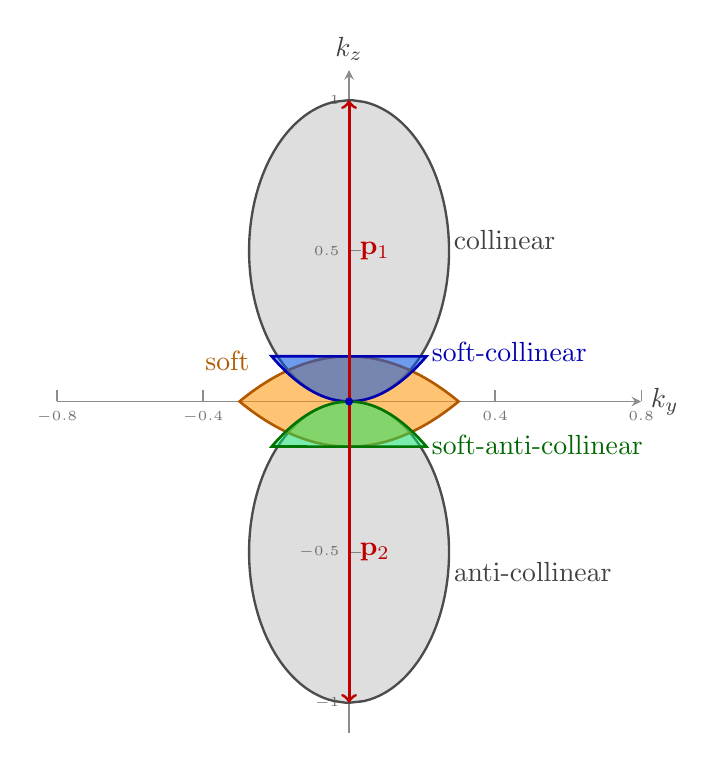
\begin{tikzpicture}
\begin{axis}[
  width=9cm,
  height=10cm,
  xmin=-0.8, xmax=0.8,
  ymin=-1.1, ymax=1.1,
  xtick distance=0.4,
  tick label style={black!55, font=\tiny},
  tick style={black!45, line width=0.45pt},
  axis lines=middle,
  axis line style={black!45, line width=0.55pt},
  xlabel={$k_y$},
  ylabel={$k_z$},
  xlabel style={anchor=west, text=black!75},
  ylabel style={anchor=south, text=black!75},
  tick align=inside,
  samples=160,
  clip=true,
]

% RegionPlot: y^2 + 0.3 z (1+z) < 0
% shifted upward by 1: plotted at vertical coordinate z+1
\path[
  fill=black!65,
  fill opacity=0.20,
  draw=black!70,
  line width=0.85pt
]
  plot[domain=-1:0, samples=180, variable=\z]
    (axis cs:{sqrt(-0.3*\z*(1+\z))},{\z+1})
  -- plot[domain=0:-1, samples=180, variable=\z]
    (axis cs:{-sqrt(-0.3*\z*(1+\z))},{\z+1})
  -- cycle;

\path[
  fill=black!65,
  fill opacity=0.20,
  draw=black!70,
  line width=0.85pt
]
  plot[domain=0:1, samples=180, variable=\z]
    (axis cs:{sqrt(0.3*\z*(1-\z))},{\z-1})
  -- plot[domain=1:0, samples=180, variable=\z]
    (axis cs:{-sqrt(0.3*\z*(1-\z))},{\z-1})
  -- cycle;

% softCollplot region 2
\path[
  fill=orange!85!yellow,
  fill opacity=0.55,
  draw=orange!70!black,
  line width=0.95pt
]
  plot[domain=-1.15:-1, samples=100, variable=\z]
    (axis cs:{sqrt(0.6*(\z+1.15))},{\z+1})
  -- plot[domain=-1:-0.85, samples=100, variable=\z]
    (axis cs:{sqrt(0.6*(-\z-0.85))},{\z+1})
  -- plot[domain=-0.85:-1, samples=100, variable=\z]
    (axis cs:{-sqrt(0.6*(-\z-0.85))},{\z+1})
  -- plot[domain=-1:-1.15, samples=100, variable=\z]
    (axis cs:{-sqrt(0.6*(\z+1.15))},{\z+1})
  -- cycle;

% softCollplot region 1
\path[
  fill=blue!65!cyan,
  fill opacity=0.50,
  draw=blue!70!black,
  line width=0.95pt
]
  plot[domain=-1:-0.85, samples=100, variable=\z]
    (axis cs:{sqrt(0.3*(\z+1))},{\z+1})
  -- plot[domain=-0.85:-1, samples=100, variable=\z]
    (axis cs:{-sqrt(0.3*(\z+1))},{\z+1})
  -- cycle;

% softCollplot2
\path[
  fill=green!55!cyan,
  fill opacity=0.45,
  draw=green!45!black,
  line width=0.95pt
]
  plot[domain=-0.15:0, samples=100, variable=\z]
    (axis cs:{sqrt(-0.3*\z)},{\z})
  -- plot[domain=0:-0.15, samples=100, variable=\z]
    (axis cs:{-sqrt(-0.3*\z)},{\z})
  -- cycle;

% Red arrows
\addplot[
  red!75!black,
  line width=1.1pt,
  ->
] coordinates {(0,0) (0,1)}
  node[midway, right, text=red!75!black] {$\mathbf{p}_1$};

\addplot[
  red!75!black,
  line width=1.1pt,
  ->
] coordinates {(0,0) (0,-1)}
  node[midway, right, text=red!75!black] {$\mathbf{p}_2$};

% Labels
\node[
  below right,
  text=orange!70!black
] at (axis cs:-0.42,0.2) {soft};

\node[
  below right,
  text=blue!70!black
] at (axis cs:0.2,0.23) {soft-collinear};

\node[
  below right,
  text=green!40!black
] at (axis cs:0.2,-0.08) {soft-anti-collinear};

\node[
  below right,
  text=black!75
] at (axis cs:0.26,0.6) {collinear};

\node[
  below right,
  text=black!75
] at (axis cs:0.26,-0.5) {anti-collinear};

% Origin marker
\addplot[
  only marks,
  mark=*,
  mark size=1.25pt,
  blue!70!black
] coordinates {(0,0)};

\end{axis}
\end{tikzpicture}


}
\end{minipage}
\begin{minipage}{0.45\textwidth}
\scalebox{0.8}{

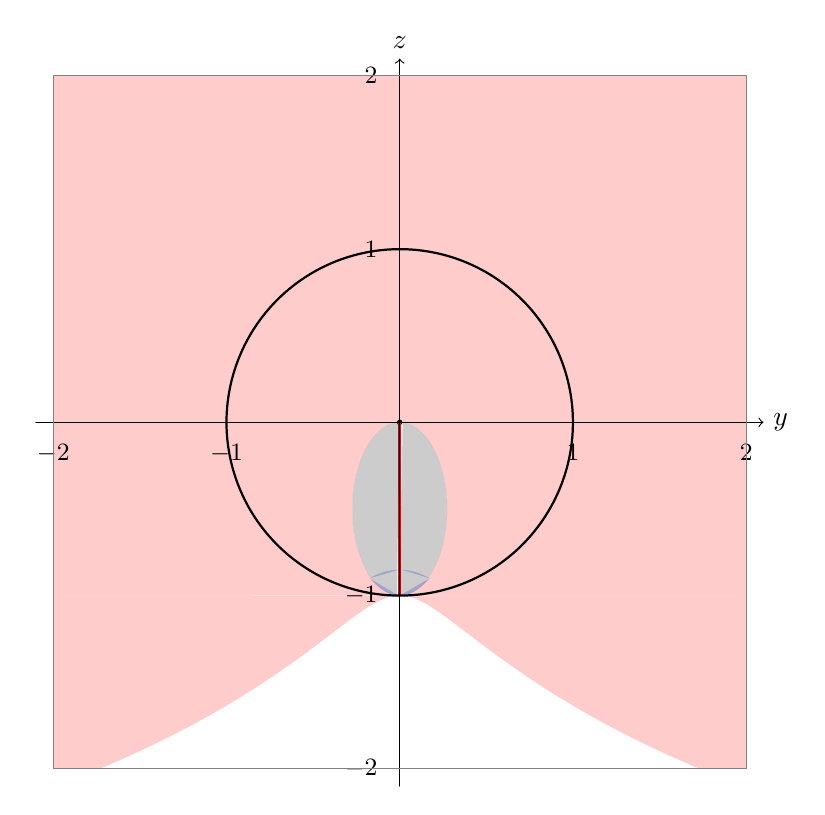
\begin{tikzpicture}[x=2.2cm,y=2.2cm,line join=round,line cap=round]
  % horizontal axis = y, vertical axis = z

  \begin{scope}
    \clip (-2,-2) rectangle (2,2);

    %========================================================
    % Red region: regpl
    %========================================================

    % For 0 <= z <= 2, the whole strip is in the red region
    \fill[red,opacity=0.20] (-2,0) rectangle (2,2);

    % For -1 <= z <= 0: outside the ellipse y^2 = -0.3 z (1+z)
    \fill[red,opacity=0.20]
      plot[domain=-1:0,samples=200]
        ({sqrt(-0.3*\x*(1+\x))},{\x})
      -- (2,0) -- (2,-1) -- cycle;

    \fill[red,opacity=0.20]
      plot[domain=0:-1,samples=200]
        ({-sqrt(-0.3*\x*(1+\x))},{\x})
      -- (-2,-1) -- (-2,0) -- cycle;

    % For -2 <= z <= -1: outside
    % y^2 = -0.3 z^2 (z+1)/(1+0.3 z)
    \fill[red,opacity=0.20]
      plot[domain=-2:-1,samples=200]
        ({sqrt(-0.3*\x*\x*(\x+1)/(1+0.3*\x))},{\x})
      -- (2,-1) -- (2,-2) -- cycle;

    \fill[red,opacity=0.20]
      plot[domain=-1:-2,samples=200]
        ({-sqrt(-0.3*\x*\x*(\x+1)/(1+0.3*\x))},{\x})
      -- (-2,-2) -- (-2,-1) -- cycle;

    %========================================================
    % Black dot shifted to the origin
    %========================================================
    \fill (0,0) circle[radius=1pt];

    %========================================================
    % Red collinear line
    %========================================================
    \draw[red,very thick] (0,0) -- (0,-1);

    %========================================================
    % Soft-collinear region: softCollplot
    % Chosen here in blue (Mathematica default-like extra color)
    %========================================================
    \fill[blue,opacity=0.20]
      (0,-1)
      plot[domain=-1:-0.9,samples=100]
        ({sqrt(0.3*(\x+1))},{\x})
      plot[domain=-0.9:-0.85,samples=100]
        ({sqrt(-0.6*\x-0.51)},{\x})
      plot[domain=-0.85:-0.9,samples=100]
        ({-sqrt(-0.6*\x-0.51)},{\x})
      plot[domain=-0.9:-1,samples=100]
        ({-sqrt(0.3*(\x+1))},{\x})
      -- cycle;

    %========================================================
    % Threshold circle: sqrt(y^2+z^2)=1
    %========================================================
    \draw[thick]
      plot[domain=0:360,samples=240]
        ({cos(\x)},{sin(\x)});

    %========================================================
    % Black collinear region: collregpl
    % y^2 + 0.3 z (1+z) < 0
    %========================================================
    \fill[black,opacity=0.20]
      plot[domain=-1:0,samples=200]
        ({sqrt(-0.3*\x*(1+\x))},{\x})
      plot[domain=0:-1,samples=200]
        ({-sqrt(-0.3*\x*(1+\x))},{\x})
      -- cycle;

  \end{scope}

  %========================================================
  % Axes
  %========================================================
  \draw[->] (-2.1,0) -- (2.1,0) node[right] {$y$};
  \draw[->] (0,-2.1) -- (0,2.1) node[above] {$z$};

  % ticks
  \foreach \t in {-2,-1,1,2}{
    \draw (\t,0.04) -- (\t,-0.04) node[below=2pt] {\small $\t$};
    \draw (0.04,\t) -- (-0.04,\t) node[left=2pt] {\small $\t$};
  }

  % optional plotting window
  \draw[gray] (-2,-2) rectangle (2,2);

\end{tikzpicture}
}
\end{minipage}
\end{figure}
\fi

\subsection{Reproducible analytic calculations}
\label{sec:reproducible-analytic-calculations}



The \href{https://github.com/ZenoCapatti/LUDY-resources}{LUDY-resources repository} hosts Python notebooks for the analytic calculations of the NLO DIS and DY cross-sections and the splitting counterterms. It also provides extensive information on installation and usage.
% Valentin PDF v2: page 10, annotation 1511.
\valentin{Will you make it public? It’s not accessible from the outside at the moment.}{\color{red} public on day ok}
%

\textbf{DIS and DY cross-sections}: the DIS and DY cross-sections are computed by generating the routed graphs and their cuts, performing the Dirac and colour algebra and reducing the scalar integrals to master integrals. In line with Reverse Unitarity, only the master integrals possessing the same cuts as the original diagram contribute. The master integrals themselves are simple and are evaluated by direct integration. The integrated results are then expanded in virtuality, to give the LP result. The computation of the parton-model diagrams is benchmarked against the DIS coefficient functions in Chapter~4 of Ref.~\cite{Bardeen:1978yd} and the Drell--Yan cross-sections of Ref.~\cite{Altarelli:1979ub}.

\textbf{Splitting counterterms}: a separate notebook derives the splitting counterterms $D_{qq}$, $D_{gq}$, $D_{qg}$, and $D_{gg}$ in the axial gauge and for arbitrary NLO processes. In the axial gauge, collinear physics is entirely contained in self-energy corrections to external legs or squared t-channel exchanges between a parton and a hard sub-process, irrespectively of the specific initial-state cuts. We start from these singular diagrams, perform the kinematic and colour algebra, expand in $\Lambda^2$ at the integrand level (using the expansion-by-regions method), and perform the transverse and $p_1^2$ integrations.  
%

\textbf{Tools}: graphs are generated with \texttt{Feyngen}~\cite{GammaLoopSoftware}), while numerator algebra is performed with \texttt{Spenso} and \texttt{Idenso}~\cite{SpensoSoftware}. All symbolic manipulations use \texttt{Symbolica}~\cite{SymbolicaSoftware}. IBP reduction is obtained with a custom python API for \texttt{Kira}~\cite{Klappert_2021}.


\subsection{Numerical performance}



Our path-finder Local Unitarity implementation \texttt{LUDY}  provides a blueprint for future high-performance implementations, including within the \href{https://github.com/alphal00p/gammaloop}{\texttt{gammaloop}} framework.
% Valentin PDF v2: page 10, annotation 1516.
\valentin{link?}
{\color{red} ok}
%
%
As expected, it underperforms established tools such as \texttt{MG5aMC}, allowing us to clearly identify two performance issues to be addressed in future work.

First, typical sample evaluation times for the integrand of the $pp\rightarrow t\bar{t}$ cross-section are about 20ms, making runs resource-intensive and time-consuming. 
% Valentin PDF v2: page 10, annotation 1527.
\valentin{Of the integrand of course, you should stress this to avoid confusion. And on what machine?
At which precision? With what stability monitoring strategy?}
%
%
This is consistent with an unoptimised implementation in Python.
% Valentin PDF v2: page 10, annotation 1533.
\valentin{But it’s not!!! I think it’s VASTLY misleading to hint at something people could understand as the implementation of the integrand being purely in Python!!!
You should be a bit more explicit about your use of efficient Symbolica evaluators, but they are stitched together with pythonic things that are slow.}
{\color{red} will improve this soon}
%
Based on our experience, using a low-level language such as Rust and managing the size of the symbolic expressions subject to evaluation could lower evaluation times by about an order of magnitude.

The second is slow convergence, which appears largely attributable to two aspects of the diagrams' soft behaviour:
\begin{itemize}
\item The variance of the integrand for the hadronic $pp\rightarrow t\bar{t}$ cross-sections increases with $\sqrt{s}$, consistent with the cancellation of double soft logarithms across graphs ($\sim$0 digits at 400~GeV and $\sim$1 digit at 2000~GeV).
% Valentin PDF v2: page 10, annotation 1542.
\valentin{I’d say the “variance of the integrand increases with $\sqrt{s}$”, it sounds a bit less superficial.}
{\color{red} ok}
%
%
A solution would be to realise the cancellation of these soft logarithms locally, by carefully aligning the phase-spaces of virtual and real emission diagrams.
%Aligning the soft phase-space regions of diagrams with soft singularities would make these cancellations local, prior to integration.
% Valentin PDF v2: page 10, annotation 1549.
\valentin{I don’t quite know what you mean or how you’d do that.
Say fine-tuning routing across graphs and adjusting parameterisation may\ldots{}}
{\color{red} ok}
%

\item The soft region, especially for infrared-finite classes containing at least one virtual diagram, involves delicate cancellations between cut diagrams and threshold counterterms (see Fig.~\ref{fig:triangle_region}). Larger weights arise in increasingly narrow regions around the soft point, yielding integrable behaviour but slowing convergence. Future high-performance implementations would need to address this through an appropriate parametrisation around the soft point.
\end{itemize}

Since our Monte Carlo implementation aimed primarily to demonstrate the correctness of the theoretical ideas presented here and lay the foundations for the numerical approach, we leave these performance issues to future work.
%


\iffalse
Our path-finder implementation of the Local Unitarity method provides a blueprint for future high-performance implementations, for example within the gammaloop framework. For this reason, and as expected, it performs poorly compared with existing tools such as \texttt{MG5}. Our numerical investigations using the path-finder implementation, however, clearly point to two performance issues that should be addressed in future work.

The first concerns evaluation time per sample. Evaluating a single sample in floating-point arithmetic for the $PP\rightarrow t\bar{t}$ cross section, for example, takes ... ms in our implementation, making runs resource-intensive and time-consuming. This timing is consistent with an unoptimised implementation in Python, a high-level programming language. An implementation in a low-level language such as Rust, together with greater attention to the size of the symbolic expressions being manipulated and evaluated, could, based on our experience, reduce evaluation times by more than an order of magnitude.

The second problem is slow convergence, which, to the best of our understanding, can largely be attributed to two main issues, both related to the soft behaviour of the diagrams we integrate:

\begin{itemize}
\item As $\sqrt{s}$ increases, the hadronic runs for $PP\rightarrow t\bar{t}$ show a clear deterioration in convergence. This is entirely consistent with the cancellation of double soft logarithms across graphs (... digits at 400~GeV and ... at 2000~GeV). The solution is to align the soft regions of phase space across the different diagrams with soft singularities, so that the cancellation occurs locally, prior to integration.

\item The soft region, especially for virtual diagrams, involves delicate cancellations between cut diagrams and threshold counterterms. Larger weights arise in increasingly narrow regions of phase space around the soft point, resulting in overall integrable behaviour that nevertheless slows convergence. A future high-performance implementation would need to address this by devising an appropriate parametrisation around the soft point.
\end{itemize}

Since the main objective of our Monte Carlo implementation was to demonstrate the correctness of the theoretical ideas presented in this paper and to lay the foundations for the numerical approach, we have chosen not to address these two issues directly, leaving their resolution to future work.
\fi

%
\end{document}
%
% ****** End of file apssamp.tex ******
